%/**
% * LaTeX thesis template (main file)
% * @author : Alexander willner <alex@willner.ws>
% * @url    : http://github.com/thesis
% */

% include config ---------------------------------------------------------------
\RequirePackage{pdf14}                 % PDF/A2-b compatibility
%\PassOptionsToPackage{demo}{graphicx} % for faster drafts
% document configuration -------------------------------------------------------
\documentclass[
        %pagesize,              % put paper size information into document
        a4paper,                % use a5paper for ISO A5; use a4paper for ISO A4
        pdftex,                 % PDF output
        %fontsize=12pt,         % font size
        headsepline,            % use headinclude also! (see M. Kohm)
        footsepline,            % use footinclude also! (see M. Kohm)
        %headinclude,            % count head to text body (not to margin)
        %footinclude,            % count foot to text body (not to margin)
        %BCOR8mm,               % set extra margin for book fixation
        headsepline,            % line on the top
        titlepage,              % show a title page
        %draft,                 % show under-/overfull boxes, hide images
        %demo=true,             % faster compile time
        %DIV=calc,              % calculate a nice type area
        %listof=totoc,          % List of Listings to ToC
        %oneside,               % e.g. same headings for odd and even pages
        %oneside=true,          % e.g. same headings for odd and even pages
        %twoside=false,         % e.g. same headings for odd and even pages
        %open=any,              % allows chapters to occur on left hand pages
        openany,               % allows chapters to occur on left hand pages
        %ngerman,               % German language support
        numbers=noendperiod    % no number at the end (German DUDEN)
%]{scrreprt}
]{book}
% ------------------------------------------------------------------------------


% lang config ------------------------------------------------------------------
\usepackage[english]{babel}                  % English language support
%\usepackage[ngerman,english]{babel}         % German language support
%\usepackage{bibgerm}                        % German bibliography support
%\usepackage[babel,german=quotes]{csquotes}  % German language support
% ------------------------------------------------------------------------------


% basic packages ---------------------------------------------------------------
%\usepackage{tocloft}                         % Tweaks for large ToCs
%\cftsetpnumwidth{2em}                        % Tweaks for large ToCs
%\usepackage[demo]{graphicx}                  % faster compile time
\input{lib/resources/config/default}          % Default config
\usepackage[
	babel,
	autostyle=true,			% automatic selection of the language specific quotation marks
	strict=true				% all warning are turned into errors
]{csquotes}                  % Biber wants it for babel

\usepackage[export]{adjustbox}                % For boxes around images
\usepackage{needspace}                        % used for embedding listings
%\usepackage{idxlayout}                       % fix index bugs and allow config
\usepackage{ifthen}			% allows for if-then-else commands

% ------------------------------------------------------------------------------

% basic config -----------------------------------------------------------------
\definecolor{LinkColor}{rgb}{0.0,0.2,0.5}     % Link color
\definecolor{MarginColor}{rgb}{0.0,0.2,0.5}   % Margin color
\definecolor{CaptionColor}{rgb}{0.0,0.2,0.5}  % Caption color
\definecolor{disabled}{gray}{0.5}             % Disabled text color
%\addtokomafont{sectioning}{\rmfamily}         % Serifs in headings
%\addtokomafont{sectioning}{\normalfont\scshape\rmfamily\color{CaptionColor}} % Serifs in headings
%\addtokomafont{sectioning}{\normalfont\rmfamily\color{CaptionColor}}        % Serifs in headings
\renewcommand{\lstlistlistingname}{List of Listings}
\renewcommand{\lstlistingname}{Listing}
\renewcommand{\contentsname}{Table of Contents}
\setcounter{secnumdepth}{4}
\setcounter{tocdepth}{2}
% basic config -----------------------------------------------------------------


% local config -----------------------------------------------------------------
\usepackage{pdflscape}
%\usepackage{subfig}
\usepackage{xmpincl}
%\includexmp{an-xmp-file-if-you-like}
\usepackage{enumitem}                   % More compact listings
\usepackage{float}                      % Provides the H float modifier option
% ------------------------------------------------------------------------------


% bibliography -----------------------------------------------------------------
\usepackage[
	autocite=inline,
	backref=true,			% backref to page with citation in references
	backrefstyle=three,		% shorten the number of displayed pages, see biblax documentation
	bibencoding=utf8,		% .bib file is utf-8 encoded
	citestyle=authoryear,		% citation stlye in text
	defernumbers=true,		% correct numbering for numerical references with multiple lists of references
	dashed=false,			% do not print dash for repeated authors
	date=year,				% only print the year in all references
	doi=true,				% print doi in references
	giveninits=true,		% abbreviate first names to initials
	hyperref=true,			% use hyperref
	isbn=true,				% print isbn in references
	maxbibnames=99,			% maximum number of authors (to avoid et al./u.a. in references
	maxcitenames=2,			% maximum number of authors in text
	sorting=nyt,			% sort in order year-name-title
	sortlocale=auto,		% sorting of the references automatically using babel
	style=authoryear-comp,		% style of the references
	uniquelist=false,		% author list is not unique (Author A, Author B, Author C = Author A et al.)	
	uniquename=false,		% see biblatex documentation (basically checks if all authors can be identified by their last name)
	url=true				% print url in the references
]{biblatex}
\addbibresource{thesis_template.bib}
\defbibheading{empty}{}
\DeclareBibliographyCategory{cited}
\AtEveryCitekey{\addtocategory{cited}{\thefield{entrykey}}}
% ------------------------------------------------------------------------------
%------------------------------
% DATE
%------------------------------
\usepackage[ngerman, english]{datetime2}

\makeatletter					% new date type of month and year only
\newcommand{\monthyeardate}{%
	\iflanguage{english}{\DTMenglishmonthname{\@dtm@month} \@dtm@year}{%
  \DTMgermanmonthname{\@dtm@month} \@dtm@year
  }
}
\makeatother	

% acronyms ---------------------------------------------------------------------
\usepackage{acro}
\acsetup{
            single=true,
            list/sort=true,
            list/template=longtable,
            index/use, %  migh result in 'pdfTeX warning (dest): name... has been referenced but does not exist, replaced by a fixed one'
            pages/display=all,
}
\robustify\footnote%
\robustify\url%

\makeatletter\newif\ifnewacro%
\@ifpackagelater{acro}{2015/08/15}{% version 2.0 or later
\setboolean{newacro}{true}
}{% else hide footnotes and citations
\setboolean{newacro}{false}
\typeout{warning: your acro package is too old (<2.0)}
}%
\makeatother

% more config ------------------------------------------------------------------
% todo: move to 'basic config'
\usepackage{lmodern}                          % Nicer fonts (for all) - times
\usepackage{mathptmx}                         % Nicer fonts (for all) - times
%\usepackage{scrhack}                         % Fix some scrbook issues
\usepackage{scrlayer-scrpage}                 % before titlesec 
%\usepackage{chapterthumb}                     % Fancy thumb index
\usepackage[chapter]{algorithm}               % Nice pseudo code
\usepackage{lettrine}                         % Drop characters, if you like
\renewcommand{\LettrineFontHook}{\color{CaptionColor}}
\usepackage[nohints]{minitoc}                 % ToC for chapters
\dominitoc[n]                                 % ToC: no caption
\renewcommand{\mtcSfont}{\small}              % ToC: small
\usepackage{makeidx}                          % Make an index
\makeindex                                    % Make an index
% ------------------------------------------------------------------------------

% chapter layout ---------------------------------------------------------------
%\usepackage[Sonny]{fncychap}                  % Nice chapter header
%\ChNameVar{\vspace*{-1in}\Large\rmfamily\vspace*{-2in}}   % Fancy chapter with serifs
%\ChTitleVar{\color{CaptionColor}\Large\rmfamily\scshape}  % Fancy chapter with serifs
\usepackage[clearempty]{titlesec}            % Suppress header and footer for empty pages
\setlength{\headheight}{1.1\baselineskip}
\titleformat{\chapter}[display]
  {\scshape\huge\color{CaptionColor}}
  {\filleft\Large\chaptertitlename~\thechapter}
  {2.5ex}
  {\titlerule\vspace{1ex}\filleft}
  [\vspace{1ex}\titlerule]
% ------------------------------------------------------------------------------

% spqueezing -------------------------------------------------------------------
%\usepackage{etoolbox}
%\makeatletter
%\patchcmd{\AC@@acro}
%  {\dotfill\pageref{acro:#1}}
%  {\nobreak\leaders\hbox{$\mkern -7mu \mkern \@dotsep mu\hbox{.}\mkern \@dotsep mu \mkern 7mu$}%
%   \hfill\nobreak\makebox[1.3em][r]{\pageref{acro:#1}}}
%  {}
%  {}
%\makeatother
% ------------------------------------------------------------------------------

% page layout ------------------------------------------------------------------
%  \usepackage[ % Optional page bleed
%    cross, # some printing services might not like it others may require it...
%    center,
%    width=216mm, % A4 + 6mm
%    height=303mm % A4 + 6mm
%  ]{crop}
\usepackage[pass,a4paper]{geometry}
%\usepackage[marginparwidth=.7in, marginparsep=0.2in]{geometry}
%\geometry{a4paper, bottom=4cm}
% \renewcommand{\topfraction}{0.9}
% \renewcommand{\bottomfraction}{0.9}
% \renewcommand{\textfraction}{0.07}         % allow minimal text w. figs
% \renewcommand{\floatpagefraction}{0.7}     % require fuller float pages
% \renewcommand{\dblfloatpagefraction}{0.7}  % require fuller float pages
% \renewcommand{\dbltopfraction}{0.9}        % fit big float above 2-col. text
% \renewcommand{\textfloatsep}{5mm}
% \setcounter{topnumber}{2}
% \setcounter{bottomnumber}{2}
% \setcounter{totalnumber}{4}                % 2 may work better
% \setcounter{dbltopnumber}{2}               % for 2-column pages
% ------------------------------------------------------------------------------


% hyperlinks (almost last package) ---------------------------------------------
\usepackage{hyperxmp}                 % Semantic meta data (RDF/XMP)
%\pdfminorversion=4                   % PDF/A compatbility
%\pdfobjcompresslevel=0               % PDF/A compatbility
%\pdfcompresslevel=0                  % PDF/A compatbility
\usepackage[pdftex,                   % Hyperlinks in PDFs
pdfa=true,                            % PDF/A compatbility (fix hyperlink with ghostscript)
pdfapart=1,                           % PDF/A compatbility
unicode=true,                         % PDF/A compatbility
raiselinks=true,			                % calculate real height of the link
breaklinks,                           % break links
%backref=page,                        % backlinks in bibliography (section, slide, page, none)
%pagebackref=true,                    % backlinks in bibliography
hyperindex=true,                      % backlinkex index
linktocpage=true,                     % ToC links pages
bookmarks=true,                       % Bookmarks for PDF viewers
bookmarksopen=true,                   % Open bookmarks
bookmarksopenlevel=2,                 % How many levels to open
bookmarksnumbered=true,               % Numbers in the bookmarks
bookmarkstype=toc,                    % Type of bookmark
plainpages=false,                     % Anchors even on plain pages?
pageanchor=true,                      % Pages are linkable
pdfstartview=FitH,                    % Open document with Fit Width
pdfpagelabels=true,                   % set PDF page labels
pdfpagemode=UseOutlines,              % Show bookmarks in viewer
colorlinks,                           % Show colored links
linkcolor=LinkColor,                  % Link color
urlcolor=LinkColor,                   % URL color
anchorcolor=LinkColor,                % Anchor color
citecolor=LinkColor,                  % Cite color
menucolor=LinkColor,                  % Menu color
hypertexnames=true                    % Whatever ;)
]{hyperref}                           % Use hyperlinks
%\renewcommand*{\backref}[1]{[cited at page #1]} % Show formatted backlinks
\usepackage{bookmark}                 % Manually add PDF bookmarks
\hypersetup{keeppdfinfo}              % fix for hyperxmp, however, breaks PDF/A compliance
% ------------------------------------------------------------------------------


% cleveref with fixes ----------------------------------------------------------
\usepackage{cleveref}                 % To ref footnotes twice (use after hyperref)
\crefformat{footnote}{#2\footnotemark[#1]#3}
% ------------------------------------------------------------------------------

% ------------------------------------------------------------------------------

%\input{lib/resources/config/commands} 				% all additional commands and options


% meta data --------------------------------------------------------------------
% meta data --------------------------------------------------------------------

%-----------------------------
% MUST BE CHANGED BY THE USER
%-----------------------------
%-----------------------------
% BOOLEAN FOR DECISION B/M THESIS OR DISSERTATION
%-----------------------------
\newboolean{isDiss}
% Options:
% true: Dissertation
% false: Bachelor/Master thesis
\setboolean{isDiss}{false}
%-----------------------------
% BOOLEAN FOR DECISION MASTER OR BACHELOR THESIS
%-----------------------------
\newboolean{isMT}
% Options:
% true: Master thesis
% false: Bachelor thesis
\setboolean{isMT}{false}
%-----------------------------
% TITLE AND AUTHOR
%-----------------------------
\newcommand{\mytitle}{This Is a Very Good Title That Illustrates What This Great Piece of Work Is All About and That Gives an Impression of What a Long Title Looks Like}
\newcommand{\firstauthor}{Antonio Günther}
\newcommand{\mymatriculationnumber}{409741}
\newcommand{\firstinitial}{AnGÜ}
\newcommand{\secondauthor}{Amandus Schnipp}
\newcommand{\secondmatriculationnumber}{409675}
\newcommand{\secondinitial}{AmSp}
\newcommand{\thirdauthor}{Elena Schnapp}
\newcommand{\thirdmatriculationnumber}{409699}
\newcommand{\thirdinitial}{ElSp}
%-----------------------------
% FOR BACHELOR/MASTER THESIS
%-----------------------------
\newcommand{\courseofstudy}{Bsc. Geotechnology}
\newcommand{\myadvisor}{Dr. Ferry Schiperski}
%-----------------------------
% KEYWORDS FOR THE ABSTRACT
%-----------------------------
\newcommand{\germankeywords}{Schlüsselwort1; Schlüsselwort2; Schlüsselwort3}
\newcommand{\englishkeywords}{Keyword1; Keyword2; Keyword3}
%-----------------------------
% FOR DISSERTATION
%-----------------------------
\newcommand{\chairman}{Prof.~Dr.-Ing.~habil.~Martina Superwichtig}
\newcommand{\firstreviewer}{\mysupervisor}
\newcommand{\secondreviewer}{Prof.~Dr.-Ing.~Hans-Georg Wichtig}
\newcommand{\dayofdefense}{\DTMdisplaydate{2020}{1}{1}{-1}}
%-----------------------------
% MUST BE CHANGED BY THE USER
%-----------------------------


%-----------------------------
% NOT TO BE CHANGED BY THE USER
%-----------------------------
\newcommand{\myuniversity}{Technische Universität Berlin}
\newcommand{\myfaculty}{Fakultät VI - Planen Bauen Umwelt}
\newcommand{\myinstitute}{Institut für Angewandte Geowissenschaften}
\newcommand{\mydepartment}{Fachgebiet Angewandte Geochemie}
\newcommand{\myplace}{Berlin}
\newcommand{\mysupervisor}{Prof.~Dr. Thomas Neumann}
\newboolean{isSG}
% Options:
% true: document in styleguide mode
% false: dissertation or thesis mode
\setboolean{isSG}{false}
\newcommand{\version}{3.3.2}
\ifthenelse{\boolean{isSG}}{\setboolean{isDiss}{true}}{}
% Subtitle English
\newcommand{\myengsubtitle}{Thesis in partial fulfillment of the requirements for the degree \\ \ifthenelse{\boolean{isMT}}{Master}{Bachelor} of Science (\ifthenelse{\boolean{isMT}}{M.Sc.}{B.Sc.})}
% Subtitle German
\newcommand{\mygersubtitle}{Wissenschaftliche Arbeit zur Erlangung des Grades \\ \ifthenelse{\boolean{isMT}}{Master}{Bachelor} of Science (\ifthenelse{\boolean{isMT}}{M.Sc.}{B.Sc.})}
%-----------------------------
% NOT TO BE CHANGED BY THE USER
%-----------------------------

%------------------------------------------
% meta from original Template
\newcommand{\metaType}{PhD of templates}
\newcommand{\metaTypeShort}{Dr.-Tmpl.}
\newcommand{\metaWhy}{To get the degree in}
\newcommand{\metaHowFinal}{Submitted}
\newcommand{\metaHowNonFinal}{Draft}
\newcommand{\metaBoard}{Board}
\newcommand{\metaSubmitted}{Presented by}
\newcommand{\metaDate}{16.~Juni~2020}
\newcommand{\metaDateEn}{16.~June~2020}
\newcommand{\metaDateExam}{\metaDate}
\newcommand{\metaNumber}{2020--06}
\newcommand{\metaTitleLayouted}{Sophisticated Template\\for a Thesis}
\newcommand{\metaTitle}{Sophisticated Template for a Thesis}
\newcommand{\metaTitleShort}{Thesis Template}
\newcommand{\metaDegree}{MTA}
\newcommand{\metaBirthplace}{Born in Foo Bar}
\newcommand{\metaAuthor}{First Last}
\newcommand{\metaAuthorMail}{first.last@example.org}
\newcommand{\metaKeywords}{Foo, Bar, First, Last}
\newcommand{\metaSubject}{Template Subject}
\newcommand{\metaUniversity}{Template University}
\newcommand{\metaFaculty}{Template Faculty}
\newcommand{\metaDepartment}{Template Department}
\newcommand{\metaCitycode}{12345}
\newcommand{\metaCity}{City}
\newcommand{\metaCountry}{Country}
\newcommand{\metaURL}{http://example.org}
\newcommand{\metaChair}{Chair}
\newcommand{\metaChairName}{Prof.\ Dr.-Ing.\ Goo Gl}
\newcommand{\metaChairUniversity}{Industry}
\newcommand{\metaReviewer}{Reviewer}
\newcommand{\metaFirstReviewerName}{Prof.\ Dr.-Ing.\ Foo Bar}
\newcommand{\metaFirstReviewerUniversity}{Example University}
\newcommand{\metaSecondReviewerName}{Prof.\ Dr.\ Bar Foo}
\newcommand{\metaSecondReviewerUniversity}{Another University}
\newcommand{\metaThirdReviewerName}{Dr.\ John Smith}
\newcommand{\metaThirdReviewerUniversity}{My University}
\newcommand{\metaFourthReviewerName}{{\color{gray}Dr.\ Jon Doe}}
\newcommand{\metaFourthReviewerUniversity}{{\color{gray}BAR}}


\newcommand{\metaAuthorShort}{\metaAuthor}
\newcommand{\metaConference}{Conference}
\newcommand{\metaConferenceArea}{Area}
\newcommand{\metaDedication}{\scriptsize{Dedicated to my beloved family.}}
% ------------------------------------------------------------------------------

\input{lib/resources/config/pdfmetadata}
% ------------------------------------------------------------------------------


% final fixes ------------------------------------------------------------------
\righthyphenmin=2
\tolerance=2000
\emergencystretch=10pt
% ------------------------------------------------------------------------------

% PDF/A color profile ----------------------------------------------------------
\immediate\pdfobj stream attr{/N 3}  file{lib/resources/pdfa/srgb.icc}% chktex 1
\pdfcatalog{%
/OutputIntents [ <<
/Type /OutputIntent
/S/GTS_PDFA1
/DestOutputProfile \the\pdflastobj\space 0 R
/OutputConditionIdentifier (sRGB IEC61966-2.1)% chktex 8
/Info(sRGB IEC61966-2.1)% chktex 8 chktex 36
>> ]
}
% ------------------------------------------------------------------------------
     % inlcude general configuration
%------------------------------
% NUMERICS
%------------------------------
\DeclareAcronym{ab}{%
	short={ab},
	long={\textbf{a}ctive \textbf{b}ound},
	short-plural={s},
	short-plural-form={abs},
	long-plural={s},
	long-plural-form={\textbf{a}ctive \textbf{b}ounds},
	tag={Numerics},
}%
\DeclareAcronym{dae}{%
	short={DAE},
	long={\textbf{D}ifferential-\textbf{a}lgebraic \textbf{e}quation (system)},
	short-plural={s},
	short-plural-form={DAEs},
	long-plural={s},
	long-plural-form={\textbf{D}ifferential-\textbf{a}lgebraic \textbf{e}quation (systems)},
	tag={Numerics},
}%
%------------------------------
% SOFTWARE
%------------------------------
\DeclareAcronym{sundials}{
	short={SUNDIALS},
	long={\textbf{Su}ite of \textbf{n}onlinear and \textbf{di}fferential-\textbf{al}gebraic equation \textbf{s}olvers},
	tag={Software},
}
%------------------------------
% whatever
%------------------------------
\DeclareAcronym{ABAC}{
	short={ABAC}, 
	long={Attributed Based Access Control}
}
\DeclareAcronym{DBpedia}{
	short={DBpedia}, 
	long={DBpedia}, 
	long-post={\acroiffirstT{\footnote{\url{http://dbpedia.org}}}}, 
	first-style = long
}
		% include abbreviations
\DeclareUnicodeCharacter{0301}{}       % fixing an UTF-8 encoding issue
%\usepackage[norefs,nocites]{refcheck} % useful, but not working with cref
%\usepackage[doublespacing]{setspace}  % useful for reviewing a printout
%\PassOptionsToPackage{cmyk}{xcolor}   % PDF/A compatibility, skipped
%\usepackage[a-2b]{pdfx}               % PDF/A compatibility, skipped
\newcommand{\isFinal}{false}            % Modify e.g. the title page
%\AddLayersToPageStyle{@everystyle@}{chapterthumb}
%\addtokomafont{chapterthumb}{\bfseries}

%------------------------------
\graphicspath{{resources/images/}} 		% directory in which LaTeX searches for figures

% ---------Draft settings--------include only required files for faster building ------------------------------
% \usepackage[demo]{graphicx}     
%\includeonly{src/03_requirements,src/06_implementation}
% ------------------------------------------------------------------------------
%------------------------------
% BEGIN DOCUMENT
%------------------------------
\begin{document}
%------------------------------
% COVER
%------------------------------
    \frontmatter
    \pagestyle{empty}
    \pagenumbering{alph}
    \pdfbookmark{Title}{title}
\newgeometry{left=35mm, right=35mm, top=35mm, bottom=35mm}

	\ifthenelse{\boolean{isDiss}}{
	%------------------------------
	% DISSERTATION COVER
	%------------------------------		
		\begin{titlepage}
			\begin{center}
				%------------------------------
				% LOGO
				%------------------------------
				\begin{minipage}{0.6\textwidth}
				\end{minipage}
				\hfill
				\begin{minipage}{0.3\textwidth}
					\centering
					\vfill
					\includegraphics[width=\textwidth]{Logo_tub}
					\vfill
				\end{minipage}
				%------------------------------
				% TITLE AND AUTHOR INFORMATION
				%------------------------------
				\vfill
				\huge\textbf{\mytitle}
				\vfill
				\Large vorgelegt von\\
				\author\\
				%------------------------------
				% UNIVERSITY
				%------------------------------
				\vfill
				von der \myfaculty \\
				der Technischen Universität Berlin\\
				zur Erlangung des akademischen Grades\\
				\vspace{0.5cm}
				Doktor der Ingenieurwissenschaften\\
				- Dr.-Ing. -\\
				\vspace{0.5cm}
				genehmigte Dissertation
			\end{center}
			\vfill
			%------------------------------
			% DOCTORAL BOARD
			%------------------------------
			\normalsize
			Promotionsausschuss:\\[2ex]
			\begin{tabular}{@{}ll}
			Vorsitzende: & \chairman \\
			1.~Gutachter: & \firstreviewer \\
			2.~Gutachter: & \secondreviewer \\
			\end{tabular}
			%------------------------------
			% DATES
			%------------------------------
			\vfill
			Tag der wissenschaftlichen Aussprache: \begin{otherlanguage}{ngerman} \dayofdefense\end{otherlanguage}
			\vfill
			\centering
			\myplace, \the\year		
		\end{titlepage}
		}{
		%------------------------------
		% THESIS COVER
		%------------------------------			
		\begin{titlepage}
			\begin{center}
				%------------------------------
				% LOGOS
				%------------------------------
				\hfill
			\parbox[t][\headheight][t]{5cm}{%
			\raggedleft
			
\includegraphics[width=0.3\textwidth]{TU-Berlin_logo}
}
				%------------------------------
				% TITLE AND AUTHOR INFORMATION
				%------------------------------
				\vfill
				\huge\textbf{\mytitle}\\[1ex]
				\Large\iflanguage{english}{\myengsubtitle}					{\iflanguage{ngerman}{\mygersubtitle}{}}\\[1ex]
				\vfill
				\normalsize
				\iflanguage{english}{in the course of studies}		{\iflanguage{ngerman}{im Studiengang}{}}\\
				\courseofstudy	
				\vfill			
				\iflanguage{english}{Submitted by:}		{\iflanguage{ngerman}{Vorgelegt von:}{}}\\
				\begin{table}[h!]
				\centering
					\begin{tabular}{@{}lrc@{}}
					\toprule
					\textbf{Co-Authors} & \textbf{Matr.Nr.} & \textbf{Initials} \\ \midrule
				          \firstauthor	& \mymatriculationnumber       	&  \firstinitial         \\
				          \secondauthor	& \secondmatriculationnumber	&  \secondinitial        \\
				          \thirdauthor 	&  \thirdmatriculationnumber	&  \thirdinitial \\
				          \bottomrule 
					\end{tabular}
				\end{table}
%				
%				\firstauthor \hfill \secondauthor \hfill \thirdauthor
%				\vfill
%				\iflanguage{english}{Matriculation numbers:}					{\iflanguage{ngerman}{Matrikelnummern:}{}}\\
%				\mymatriculationnumber \hfill \secondmatriculationnumber \hfill \thirdmatriculationnumber
				%------------------------------
				% DEPARTMENT AND UNIVERSITY
				%------------------------------
				\vfill	
				\normalsize
				\iflanguage{english}{Under the scientific supervision of}{\iflanguage{ngerman}{Unter der wissenschaftlichen Leitung von}{}}\\
				\textbf{\mysupervisor}
				\vfill
				\iflanguage{english}{Under the scientific guidance of}{\iflanguage{ngerman}{Unter der wissenschaftlichen Betreuung von}{}}\\
				\textbf{\myadvisor}
				\vfill
				\myplace, \monthyeardate
				\vfill
				\myuniversity\\
				\myfaculty\\
				\myinstitute\\
				\mydepartment\\
			\end{center}				
		\end{titlepage}
		}

\restoregeometry%
%\end{titlepage}

    \cleardoublepage\iflanguage{english}{
	\chapter*{Affidavit}
	}{\iflanguage{ngerman}{
		\chapter*{Eidesstattliche Erklärung}
		}{}
	}
%------------------------------
% GERMAN
%------------------------------
\begin{otherlanguage}{ngerman}
\begin{itemize}[label={\checkmark}]
\item Die Arbeit enthält eine deutsche Zusammenfassung.  
\item Die Arbeit enthält eine englische Zusammenfassung.
\item  Die Arbeit enthält eine Selbständigkeitserklärung nach § 60 Abs. 8 AllgStuPO:
\end{itemize}
Hiermit erkläre ich an Eides statt, dass ich die vorliegende Arbeit selbstständig und eigenhändig sowie ausschließlich unter Verwendung der aufgeführten Quellen und Hilfsmittel angefertigt habe.\\[1cm]
\makebox[3in][l]{\hrulefill}\\
\textsc{\firstauthor} \\
\myplace, \monthyeardate
\end{otherlanguage}
\vfill
%------------------------------
% ENGLISH
%------------------------------
\begin{otherlanguage}{english}
\begin{itemize}[label={\checkmark}]
\item The thesis contains a German abstract.   
\item The thesis contains an English abstract. 
\item The thesis includes a declaration that I completed the work independently in accordance with section § 60 Abs. 8 AllgStuPO:
\end{itemize}
I hereby confirm that I prepared this thesis independently and by exclusive reliance on literature or tools indicated herein.\\[1cm]
\makebox[3in][l]{\hrulefill}\\
\textsc{\firstauthor} \\
\myplace, \monthyeardate
\end{otherlanguage}
%------------------------------
% PREMATTER
%------------------------------
    \pagestyle{scrheadings}
    %\lohead[]{}
    \pagenumbering{roman}
    \setcounter{page}{1}
    \pdfbookmark{Acknowledgments}{acknowledgments}
\chapter*{Acknowledgments}

\todomid{thank your supervisors}

\todomid{thank your colleagues}

\todomid{thank your family and friends}

\vspace{0.5in}
\begin{flushright}
  \myplace, \monthyeardate%
\end{flushright}
\cleardoublepage{}
    \pdfbookmark{Abstract}{abstract}
\chapter*{Abstract}

{\setlength{\parindent}{-.1cm}%
\sidenote{Research Area:\\Foo Bar}%
\todomid{write about the research area}

\sidenote{Application Area:\\Bar Foo}
\todomid{write about the application area}

\sidenote{Research Issue:\\Foo Fooli}
\todomid{write about the research issue}

\sidenote{Own Approach:\\Bar Barli}
\todomid{write about the own approach}

\sidenote{Scientific Contributions}
\todomid{write about the scientific contributions}

\sidenote{Validation \& Outlook}
\todomid{write about the validation and outlook}

\cleardoublepage
\begin{otherlanguage}{ngerman}
\pdfbookmark{Zusammenfassung}{Zusammenfassung}
\chapter*{Zusammenfassung}%

\sidenote{For\-schungs\-be\-reich:\\Foo Bar}%
\todomid{write}

\sidenote{Ein\-grenz\-ung:\\Bar Foo}
\todomid{write}

\sidenote{Pro\-blem\-stel\-lung:\\Foo Fooli}
\todomid{write}

\sidenote{Eigener Ansatz:\\Bar Barli}
\todomid{write}

\sidenote{Wis\-sen\-schaft\-lich\-er Bei\-trag}
\todomid{write}

\sidenote{Va\-li\-die\-rung \& Aus\-blick}
\todomid{write}

\end{otherlanguage}

}
\cleardoublepage
\cleardoublepage
%------------------------------
% LISTS OF...
%------------------------------
    \phantomsection
    % Change the depth for review
\pdfbookmark{Table of Contents}{toc}
\renewcommand{\contentsname}{Table of Contents}
\tableofcontents

\cleardoublepage
\phantomsection\addstarredchapter{\listfigurename}
\listoffigures

\cleardoublepage
\phantomsection\addstarredchapter{\lstlistlistingname}
\lstlistoflistings

\cleardoublepage
\phantomsection\addstarredchapter{\listtablename}
\listoftables

%\cleardoublepage
%\phantomsection\addstarredchapter{\abbrevname}
%\input{00_abbreviations}

\cleardoublepage
\cleardoublepage
%------------------------------
% CONTENT
%------------------------------
    \mainmatter
    %\lohead[\putchapterthumb]{\putchapterthumb}
    \pagenumbering{arabic}
    \setcounter{page}{1}
    %\linenumbers
    \acresetall%
    %\cleardoublepage\chapter{Introduction}
\minitoc\label{sec:introduction}\vspace{.5cm}

\section{Background and Motivation}

\sidenote{Research Context: Foo}
\todomid{write about the research context \gls{Foo}}\index{Foo}

\sidenote{Research Area: Bar}
\todomid{write about the research area and \Cref{fig:intro:a}}\index{Bar}

\begin{figure}[H]
    \centering
    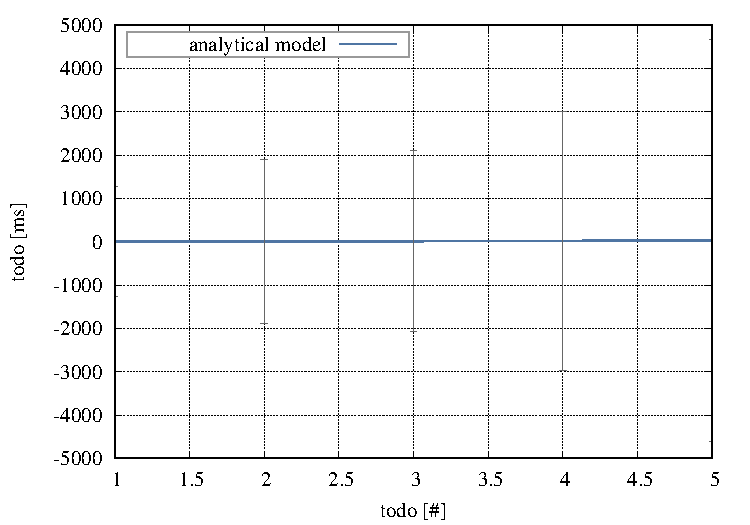
\includegraphics[width=.55\textwidth]{resources/images/example1}
    \caption{Example (based on~\cite{li2002design})}\label{fig:intro:a}
\end{figure}

\sidenote{Application Area: Foo Fooli}\index{Foo!Fooli}
\todomid{write about the application area~\cite{Heflin2004}}

\begin{figure}[H]
      \centering
      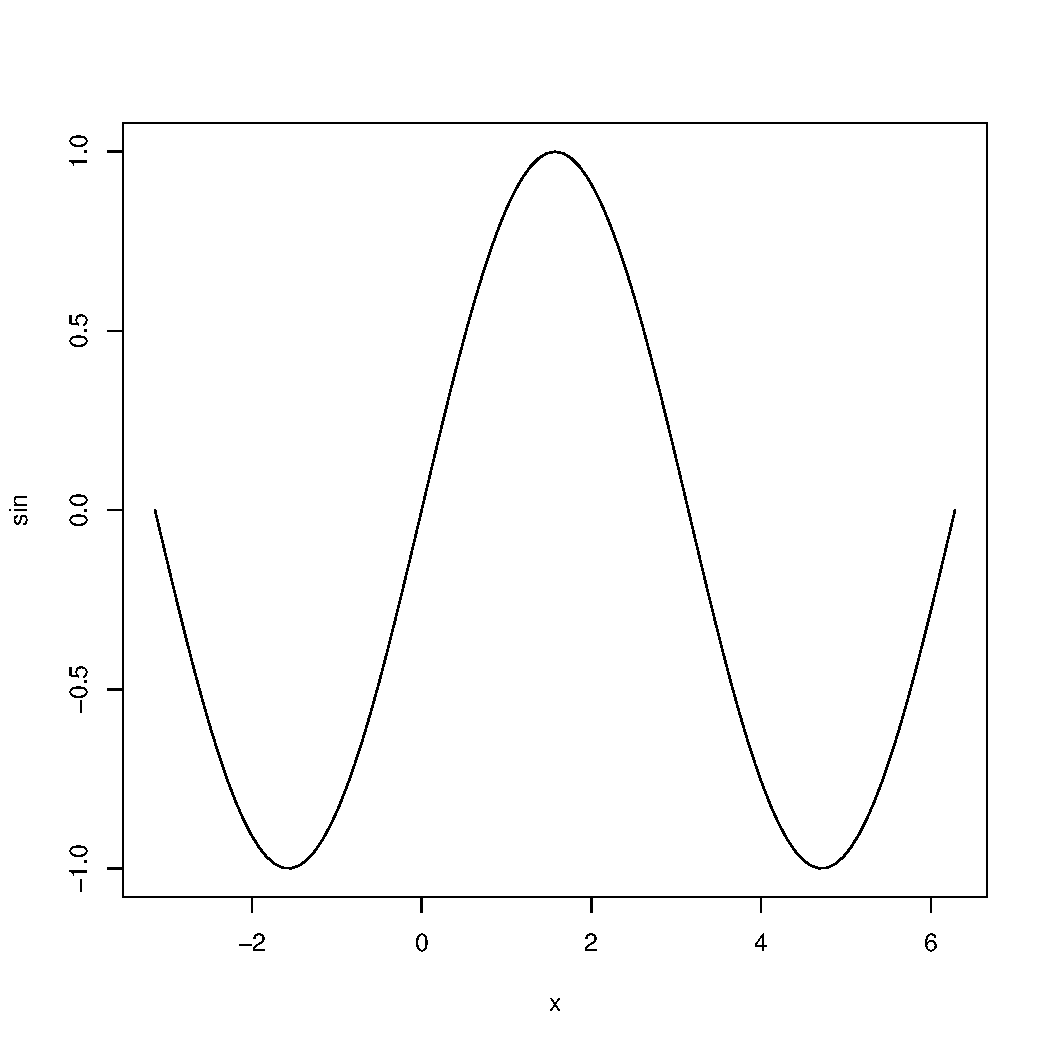
\includegraphics[width=.45\textwidth]{resources/images/example2}
      \caption{Another example~\cite{li2002design}}\label{fig:intro:b}
\end{figure}

\sidenote{Research Focus: Bar Barli}\index{Bar!Barli}
\todomid{write about the research focus and \Cref{fig:intro:b}}

\sidenote{Taxonomy}\index{Taxonomy}
\todomid{write about the taxonomy and \ac{ABAC}}

\begin{figure}[htbp]
      \centering
      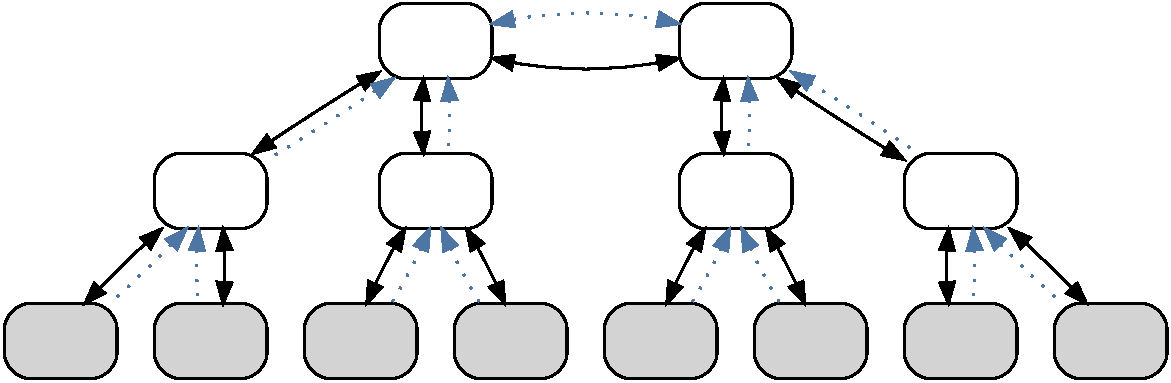
\includegraphics[width=.75\textwidth]{resources/images/example3}
      \caption{Taxonomy}
\end{figure}

\section{Problem Statement}\index{Requirements}

\sidenote{State of the Art}
\todomid{write about the State of the Art}

\sidenote{Issue:\\Example 1}
\todomid{write about the first issue}

\sidenote{Issue:\\Example 2}
\todomid{write about the second issue}

\sidenote{Synopsis}
\todomid{write about the synopsis of the issues and \Cref{fig:intro:c}}

\begin{figure}[htbp]
    \centering
    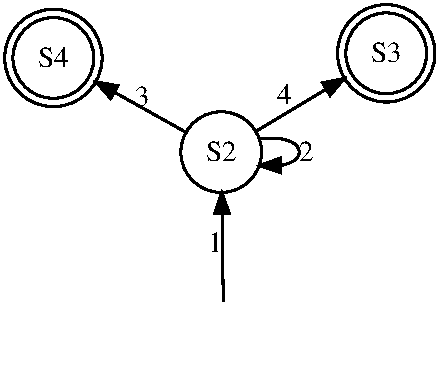
\includegraphics[width=.5\textwidth]{resources/images/job_lifecycle}
    \caption{Relationship between issues}\label{fig:intro:c}
\end{figure}

\section{Assumptions and Scope}

\sidenote{Research Assumptions}
\todomid{write about the research assumptions~\cite{li2002design}}

\sidenote{Research Scope}
\todomid{write about the research scope --- \Cref{fig:intro:a,fig:intro:b,fig:intro:c}}


\section{Objectives and Contributions}

\begin{figure}[htbp]
    \centering
    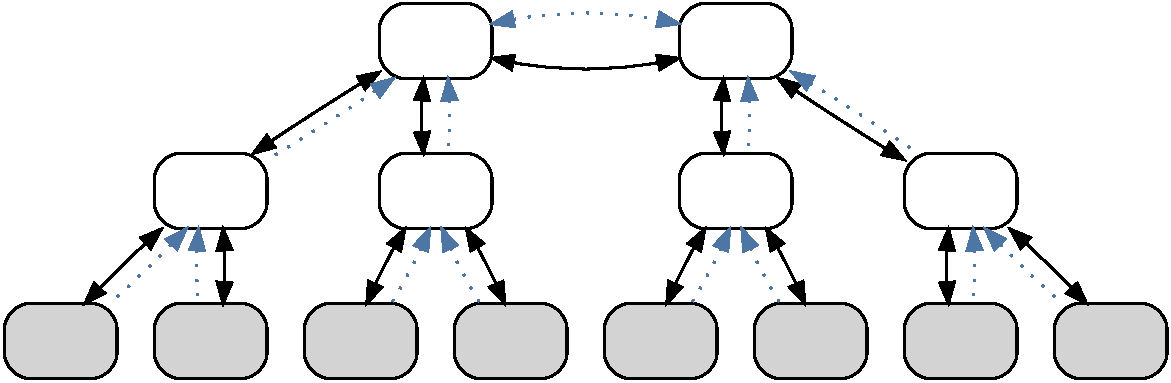
\includegraphics[width=.55\textwidth]{resources/images/example3}
    \caption{Structure of research}\label{fig:intro:struct}
\end{figure}

\sidenote{Research Objectives \& Contributions}
\todomid{write about the research objectives and \ac{DBpedia} and \Cref{fig:intro:struct}}

\section{Methodology and Outline}

\todomid{write about the research outline and \Cref{fig:intro:methodology}. Summarize \Cref{sec:introduction,sec:sota,sec:reqs,sec:contrib1,sec:contrib2,sec:contrib3,sec:eval,sec:summary}.}

\begin{sidewaysfigure}
    \centering
    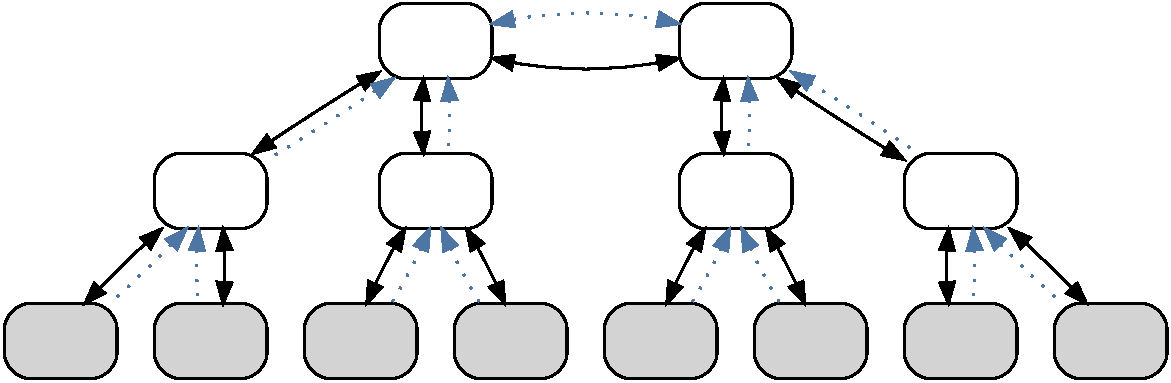
\includegraphics[width=.7\textwidth]{resources/images/example3}
    \caption{Workflow of the research and structure of the thesis}\label{fig:intro:methodology}
\end{sidewaysfigure}

    \cleardoublepage\chapter{State of the Art}\label{sec:sota}\minitoc\vspace{.5cm}\index{SotA}

\section{Introduction}

\begin{wrapfigure}{r}{0.2\textwidth}
    \centering
    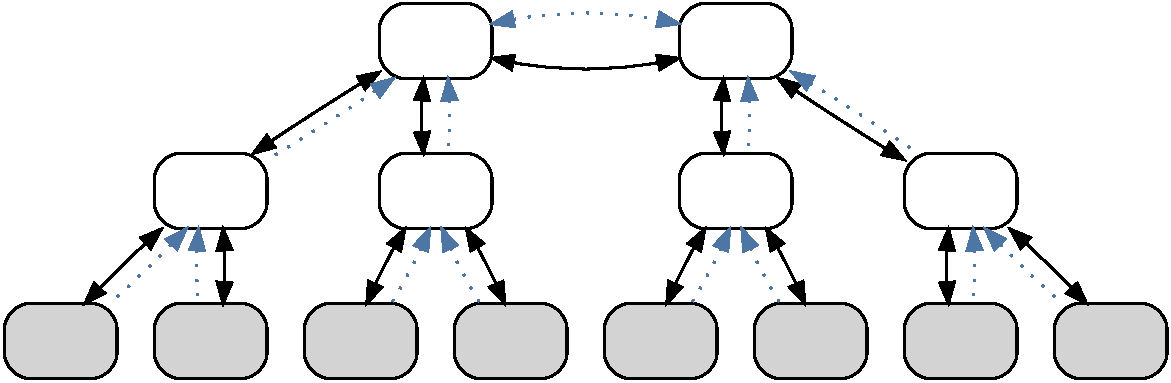
\includegraphics[width=0.2\textwidth]{resources/images/example3}
\end{wrapfigure}

\sidenote{Overview}
\todomid{write}

\section{Related Area 1}\index{Related Area}

\begin{figure}[H]
    \centering
    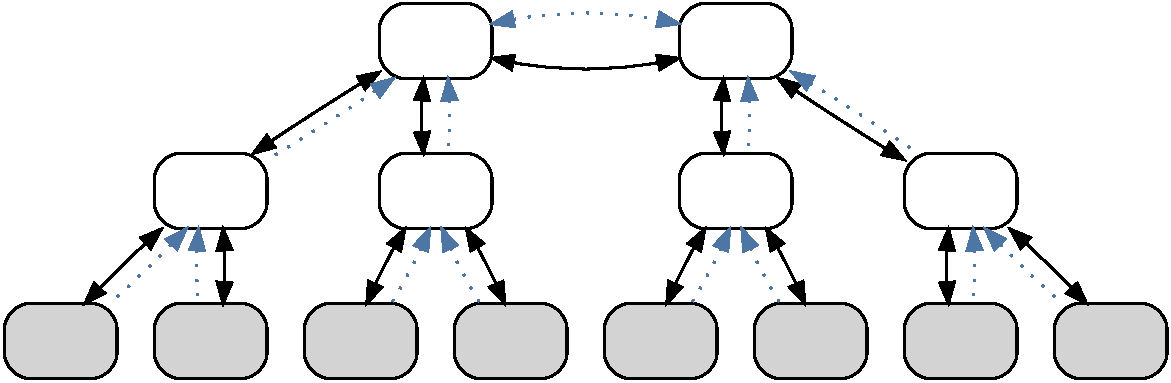
\includegraphics[width=.55\textwidth]{resources/images/example3}
    \caption{Related area 1 within the structure of research}\label{fig:hourglass:ra1}
\end{figure}

\sidenote{Overview}
\todomid{write about \Cref{fig:hourglass:ra1}}

\sidenote{Focus}
oder auch Abkürzungen wie \ac{ab} und \ac{dae}.

\subsection{Specific Example 1}

\sidenote{Definition}
\todomid{write}

\sidenote{Issues}
\todomid{write}

\subsection{Specific Example 2}

\sidenote{Definition}
Irgendein Text mit acronymen \ac{ABAC}	\autocite{Auer2007}, oder \ac{sundials} oder \ac{DBpedia} \cite{li2002design,Yuan2005}

\sidenote{Implementations}
\todomid{write}

\sidenote{Research}
Wiederhole ein zwei Abkürzungen wie \ac{sundials} oder \ac{DBpedia}


\sidenote{Standards}
\todomid{write}

\sidenote{Adoption}
\todomid{write}

\subsection{Specific Example 3}\index{Example 3}

\sidenote{Transition}
\todomid{write about \Cref{fig:sota:trans}}

\begin{figure}
    \centering
    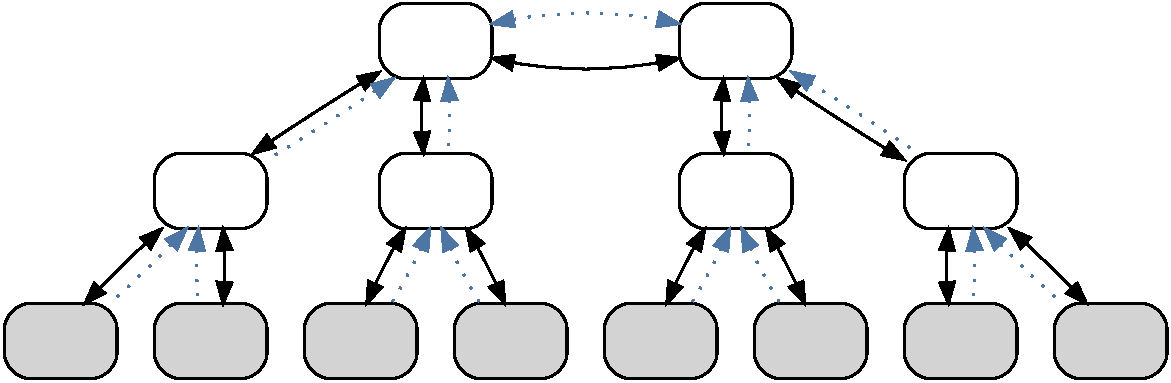
\includegraphics[width=.85\textwidth]{resources/images/example3}
    \caption{Comparison of Example 2 and Example 3 (based on~\cite{li2002design})}\label{fig:sota:trans}
\end{figure}

\sidenote{Standards}
\todomid{write}

\sidenote{Extension}
\todomid{write}

\sidenote{Other Standards}
\todomid{write}

\sidenote{Something}
\todomid{write}

\sidenote{Something}
\todomid{write}

\sidenote{Something}
\todomid{write}

\sidenote{Something}
\todomid{write}

\sidenote{Something}
\todomid{write}

\sidenote{Something}
\todomid{write}

\section{Related Area 2}\index{Related Area 2}

\sidenote{Overview}
\todomid{write}

\sidenote{Focus}
\todomid{write about \Cref{fig:sota:ra2}}

\begin{figure}[!hbtp]
    \centering
    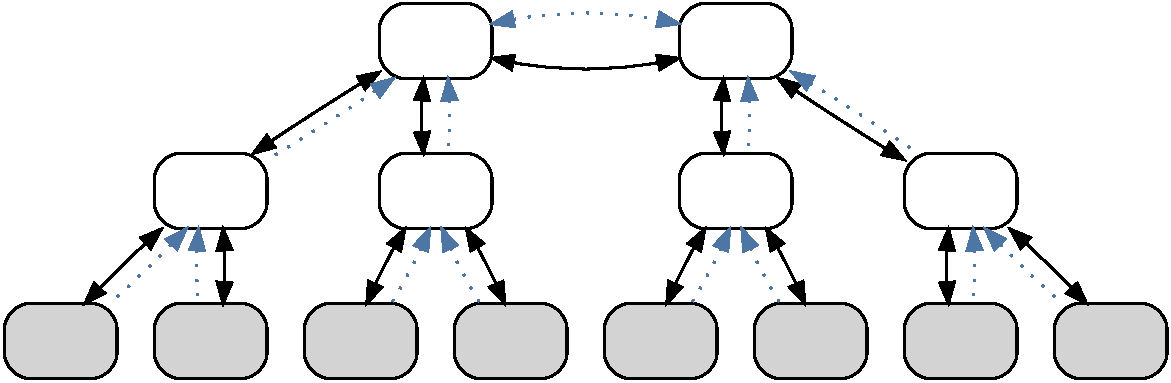
\includegraphics[width=1\textwidth]{resources/images/example3}
    \caption{Related Area 2}\label{fig:sota:ra2}
\end{figure}

\sidenote{Something}
\todomid{write}

\subsection{Specific Example 1}

\sidenote{Definition}
\todomid{write}

\sidenote{Issues}
\todomid{write}

\subsection{Specific Example 2}

\sidenote{Definition}
\todomid{write}

\sidenote{Implementations}
\todomid{write}

\sidenote{Research}
\todomid{write}

\sidenote{Standards}
\todomid{write}

\sidenote{Adoption}
\todomid{write}


\section{Related Area 3}\index{Related Area 3}

\sidenote{Overview}
\todomid{write}

\sidenote{Focus}
\todomid{write about \Cref{fig:sota:ra3}}

\begin{figure}[!hbtp]
    \centering
    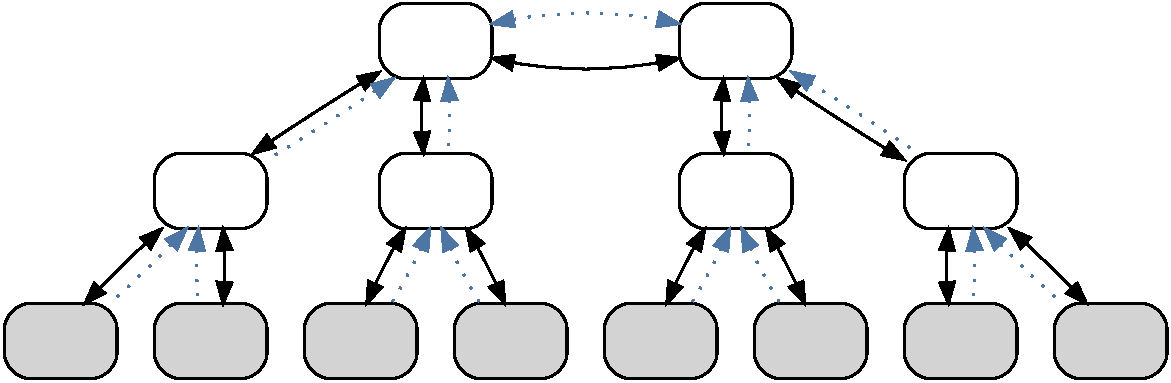
\includegraphics[width=1\textwidth]{resources/images/example3}
    \caption{Related Area 3}\label{fig:sota:ra3}
\end{figure}

\sidenote{Something}
\todomid{write}

\subsection{Specific Example 1}

\sidenote{Definition}
\todomid{write}

\sidenote{Issues}
\todomid{write}

\subsection{Specific Example 2}

\sidenote{Definition}
\todomid{write}

\sidenote{Implementations}
\todomid{write}

\sidenote{Research}
\todomid{write}

\sidenote{Standards}
\todomid{write}

\sidenote{Adoption}
\todomid{write}

\section{Conclusion}

\sidenote{Summary}
\todomid{write}

\sidenote{Takeaway 1}
\todomid{write}

\sidenote{Takeaway 2}
\todomid{write}

\sidenote{Takeaway 3}
\todomid{write}

\sidenote{Next chapter}
\todomid{write}

%    \cleardoublepage
\chapter{Requirement Analysis}\label{sec:reqs}\minitoc\vspace{.5cm}
\index{Requirements}

\section{Introduction}

\begin{wrapfigure}{r}{0.2\textwidth}
    \centering
    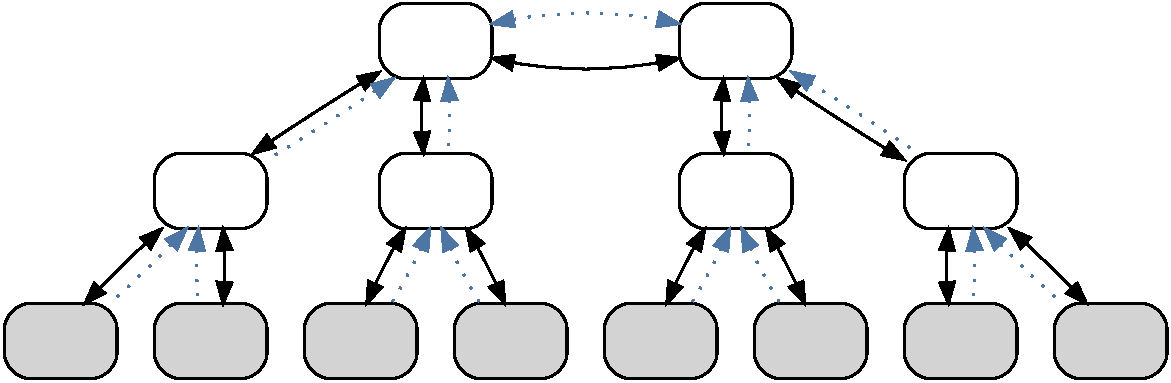
\includegraphics[width=0.2\textwidth]{resources/images/example3}
\end{wrapfigure}

\sidenote{Overview}
\todomid{write about \Cref{fig:req:details}}

\begin{figure}[H]
    \centering
    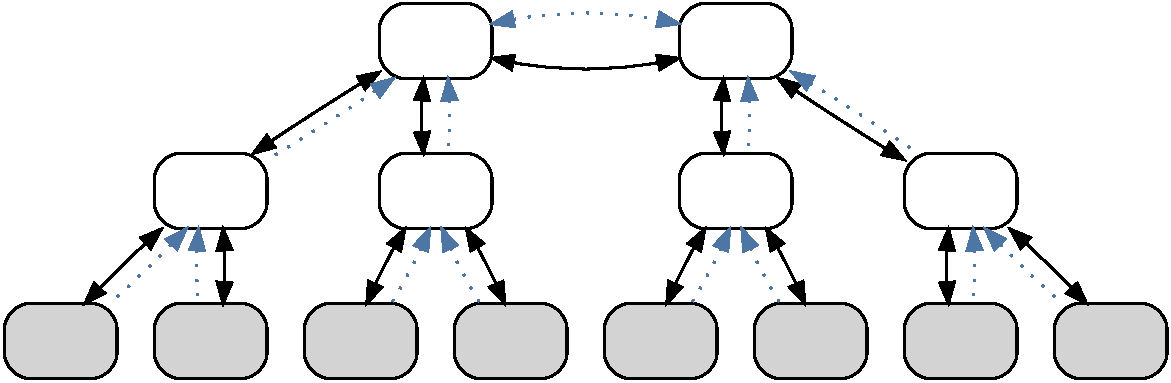
\includegraphics[width=.85\textwidth]{resources/images/example3}
    \caption{More detailed overview of the requirements}\label{fig:req:details}
\end{figure}

\sidenote{Structure of Research}
\todomid{write about \Cref{fig:hourglass:reqs}}

\begin{figure}[H]
    \centering
    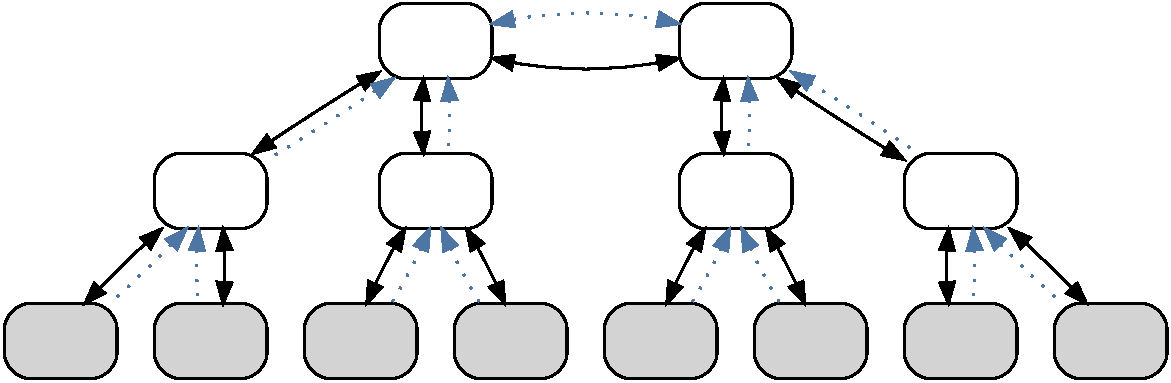
\includegraphics[width=.55\textwidth]{resources/images/example3}
    \caption{Placement of the requirement section in the structure of research}\label{fig:hourglass:reqs}
\end{figure}

\section{Stakeholder 1}

\sidenote{\Cref{tbl:reqs:stakeholder1}}
\todomid{write about \Cref{tbl:reqs:stakeholder1}}

\begin{tabularx}{\textwidth}{lX}
    \caption{Requirements from stakeholder 1 perspective}\label{tbl:reqs:stakeholder1}\\
    \toprule
    \textbf{\#}& \textbf{Description}  \\\midrule
    \endfirsthead%
    \toprule
    \textbf{\#}& \textbf{Description}  \\\midrule
    \endhead%
    \requirement{U}{req:stakeholder1:foo}{Foo}
       & \todomid{write}
    \\\midrule
    \requirement{U}{req:stakeholder1:bar}{Bar}
       & \todomid{write}
    \\\bottomrule
\end{tabularx}

\section{Stakeholder 2}

\sidenote{\Cref{tbl:reqs:stakeholder2}}
\todomid{write about \Cref{tbl:reqs:stakeholder2}}

\begin{tabularx}{\textwidth}{lX}
    \caption{Requirements from stakeholder 2 perspective}\label{tbl:reqs:stakeholder2}\\
    \toprule
    \textbf{\#}& \textbf{Description}  \\\midrule
    \endfirsthead%
    \toprule
    \textbf{\#}& \textbf{Description}  \\\midrule
    \endhead%
    \requirement{S}{req:stakeholder2:foo}{Foo}
       & \todomid{write}
    \\\midrule
    \requirement{S}{req:stakeholder2:bar}{Bar}
       & \todomid{write}
    \\\bottomrule
\end{tabularx}

\section{Stakeholder 3}

\sidenote{\Cref{tbl:reqs:stakeholder3}}
\todomid{write about \Cref{tbl:reqs:stakeholder3}}

\begin{tabularx}{\textwidth}{lX}
    \caption{Requirements from stakeholder 3 perspective}\label{tbl:reqs:stakeholder3}\\
    \toprule
    \textbf{\#}& \textbf{Description}  \\\midrule
    \endfirsthead%
    \toprule
    \textbf{\#}& \textbf{Description}  \\\midrule
    \endhead%
    \requirement{T}{req:stakeholder3:foo}{Foo}
       & \todomid{write}
    \\\midrule
    \requirement{T}{req:stakeholder3:bar}{Bar}
       & \todomid{write}
    \\\bottomrule
\end{tabularx}

\section{Conclusion}

\sidenote{Summary}
\todomid{write}

\sidenote{Takeaway 1}
\todomid{write}

\sidenote{Takeaway 2}
\todomid{write}

\sidenote{Takeaway 3}
\todomid{write}

\sidenote{Next chapter}
\todomid{write}

%    \cleardoublepage
\chapter{Contribution 1}\label{sec:contrib1}\minitoc\vspace{.5cm}
\index{Contribution 1}

\section{Introduction}

\begin{wrapfigure}{r}{0.2\textwidth}
    \centering
    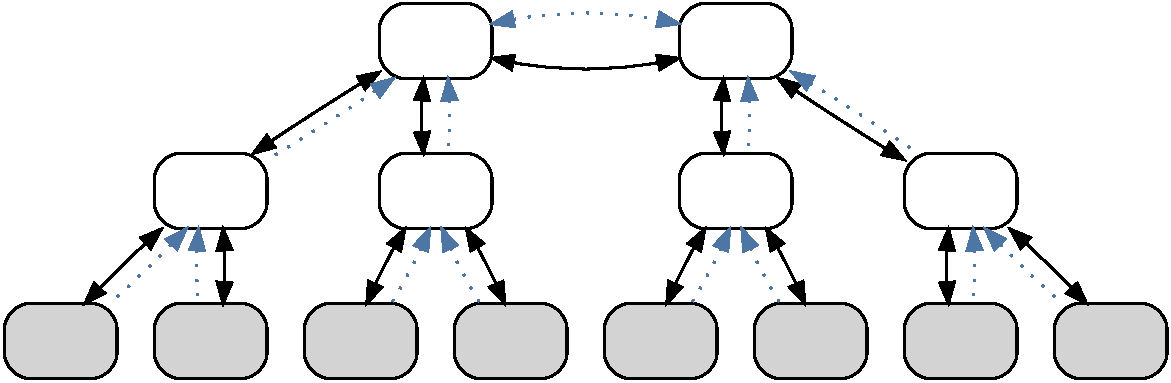
\includegraphics[width=0.2\textwidth]{resources/images/example3}
\end{wrapfigure}

\sidenote{Overview}
\todomid{write}

\sidenote{Structure of Research}
\todomid{write about \Cref{fig:hourglass:contrib1}}

\begin{figure}[H]
    \centering
    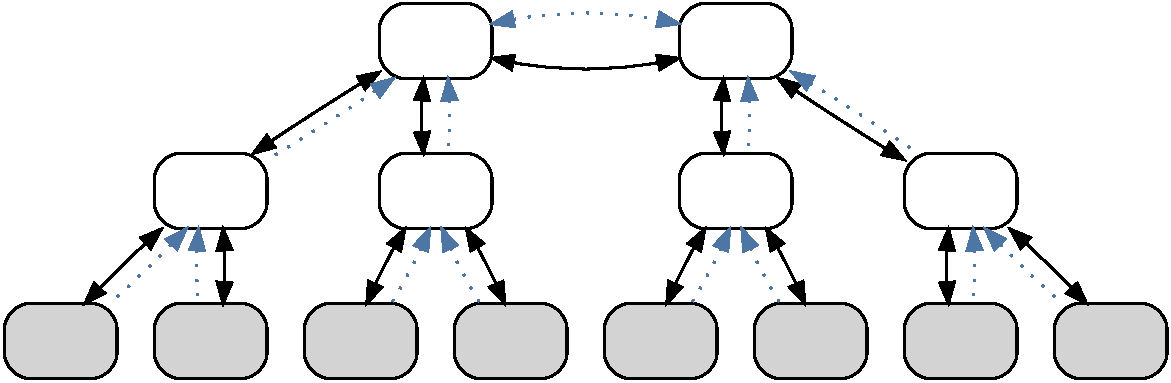
\includegraphics[width=.55\textwidth]{resources/images/example3}
    \caption{Placement of contribution 1 in the structure of research}\label{fig:hourglass:contrib1}
\end{figure}

\section{State of the Art}

\sidenote{Overview}
\todomid{write about \Cref{fig:contrib1:related}}

\begin{figure}[htbp]
    \centering
    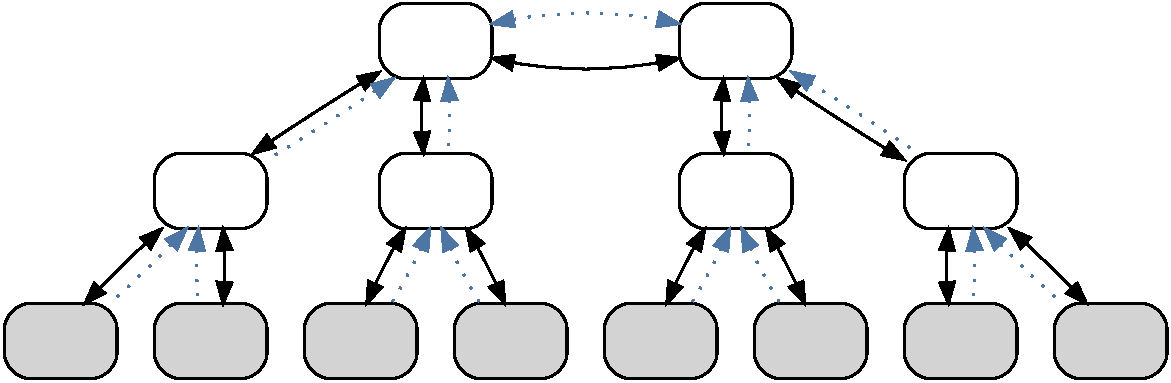
\includegraphics[width=.6\textwidth]{resources/images/example3}
    \caption{Relationship of contribution 1 to related work}\label{fig:contrib1:related}
\end{figure}

\subsection{Related Work 1}

\sidenote{Overview}
\todomid{write}

\sidenote{Some Aspects}
\todomid{write}

\sidenote{Issues}
\todomid{write about \Cref{lst:contrib1:rw1}}

\lstset{caption=Listing related to related work 1 for contribution 1, label=lst:contrib1:rw1,
language=xml, breaklines=true, numbers=left, basicstyle=\small\ttfamily,
stepnumber=1, frame=single, inputencoding=utf8/latin1}~\lstinputlisting{resources/code/example.java}

\subsection{Related Work 2}

\sidenote{Overview}
\todomid{write}

\sidenote{Some Aspects}
\todomid{write}

\sidenote{Issues}
\todomid{write about \Cref{lst:contrib1:rw2}}

\lstset{caption=Listing related to related work 2 for contribution 1, label=lst:contrib1:rw2,
language=xml, breaklines=true, numbers=left, basicstyle=\small\ttfamily,
stepnumber=1, frame=single, inputencoding=utf8/latin1}~\lstinputlisting{resources/code/example.java}

\subsection{Related Work 3}

\sidenote{Overview}
\todomid{write}

\sidenote{Some Aspects}
\todomid{write}

\sidenote{Issues}
\todomid{write about \Cref{lst:contrib1:rw3}}

\lstset{caption=Listing related to related work 3 for contribution 1, label=lst:contrib1:rw3,
language=xml, breaklines=true, numbers=left, basicstyle=\small\ttfamily,
stepnumber=1, frame=single, inputencoding=utf8/latin1}~\lstinputlisting{resources/code/example.java}


\section{Own Approach}

\subsection{Overview}

\sidenote{Intro}
\todomid{write}

\sidenote{Goal}
\todomid{write about \Cref{fig:contrib1:goal}}

\begin{figure}[htbp]
    \centering
    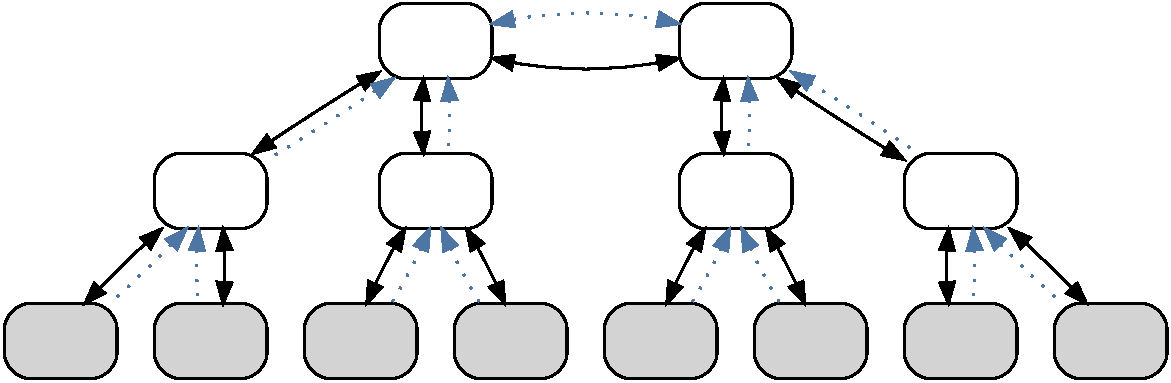
\includegraphics[width=.95\textwidth]{resources/images/example3}
    \caption{Contribution 1 goal}\label{fig:contrib1:goal}
\end{figure}

\sidenote{Approach}
\todomid{write}

\subsection{First Part}

\sidenote{Overview}
\todomid{write}

\sidenote{Approach}
\todomid{write}

\sidenote{Integration}
\todomid{write}

\subsection{Second Part}

\sidenote{Overview}
\todomid{write}

\sidenote{Approach}
\todomid{write}

\sidenote{Integration}
\todomid{write}

\subsection{Third Part}

\sidenote{Overview}
\todomid{write}

\sidenote{Approach}
\todomid{write}

\sidenote{Integration}
\todomid{write}

\section{Conclusion}

\sidenote{Summary}
\todomid{write}

\sidenote{Takeaway 1}
\todomid{write}

\sidenote{Takeaway 2}
\todomid{write}

\sidenote{Takeaway 3}
\todomid{write}

\sidenote{Next chapter}
\todomid{write}

%    \cleardoublepage
\chapter{Contribution 2}\label{sec:contrib2}\minitoc\vspace{.5cm}
\index{Contribution 2}

\section{Introduction}

\begin{wrapfigure}{r}{0.2\textwidth}
    \centering
    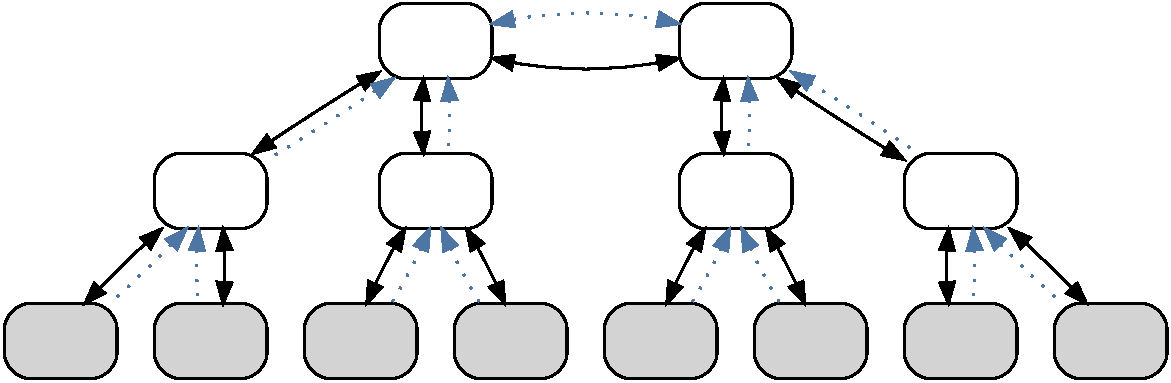
\includegraphics[width=0.2\textwidth]{resources/images/example3}
\end{wrapfigure}

\sidenote{Overview}
\todomid{write}

\sidenote{Structure of Research}
\todomid{write about \Cref{fig:hourglass:contrib2}}

\begin{figure}[H]
    \centering
    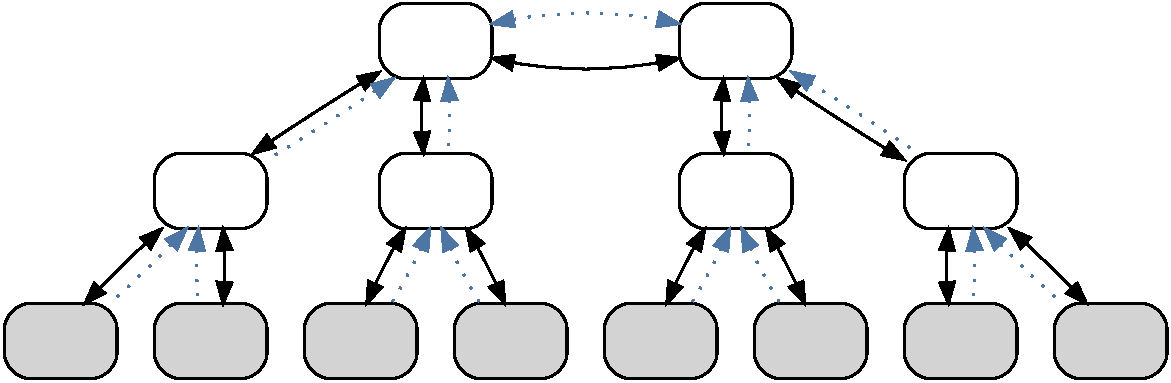
\includegraphics[width=.55\textwidth]{resources/images/example3}
    \caption{Placement of Contribution 2 in the structure of research}\label{fig:hourglass:contrib2}
\end{figure}

\section{State of the Art}

\sidenote{Overview}
\todomid{write about \Cref{fig:contrib2:related}}

\begin{figure}[htbp]
    \centering
    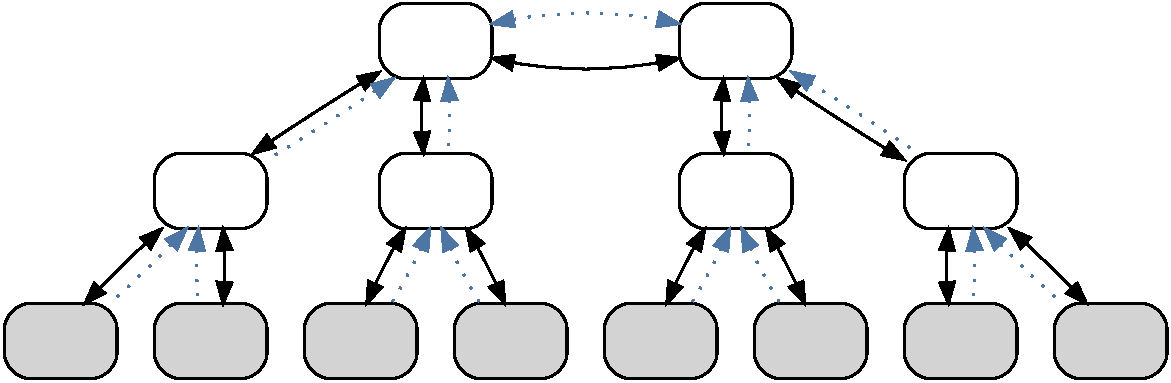
\includegraphics[width=.6\textwidth]{resources/images/example3}
    \caption{Relationship of Contribution 2 to related work}\label{fig:contrib2:related}
\end{figure}

\subsection{Related Work 1}

\sidenote{Overview}
\todomid{write}

\sidenote{Some Aspects}
\todomid{write}

\sidenote{Issues}
\todomid{write about \Cref{lst:contrib2:rw1}}

\lstset{caption=Listing related to related work 1 for Contribution 2, label=lst:contrib2:rw1,
language=xml, breaklines=true, numbers=left, basicstyle=\small\ttfamily,
stepnumber=1, frame=single, inputencoding=utf8/latin1}~\lstinputlisting{resources/code/example.java}

\subsection{Related Work 2}

\sidenote{Overview}
\todomid{write}

\sidenote{Some Aspects}
\todomid{write}

\sidenote{Issues}
\todomid{write about \Cref{lst:contrib2:rw2}}

\lstset{caption=Listing related to related work 2 for Contribution 2, label=lst:contrib2:rw2,
language=xml, breaklines=true, numbers=left, basicstyle=\small\ttfamily,
stepnumber=1, frame=single, inputencoding=utf8/latin1}~\lstinputlisting{resources/code/example.java}

\subsection{Related Work 3}

\sidenote{Overview}
\todomid{write}

\sidenote{Some Aspects}
\todomid{write}

\sidenote{Issues}
\todomid{write about \Cref{lst:contrib2:rw3}}

\lstset{caption=Listing related to related work 3 for Contribution 2, label=lst:contrib2:rw3,
language=xml, breaklines=true, numbers=left, basicstyle=\small\ttfamily,
stepnumber=1, frame=single, inputencoding=utf8/latin1}~\lstinputlisting{resources/code/example.java}


\section{Own Approach}

\subsection{Overview}

\sidenote{Intro}
\todomid{write}

\sidenote{Goal}
\todomid{write about \Cref{fig:contrib2:goal}}

\begin{figure}[htbp]
    \centering
    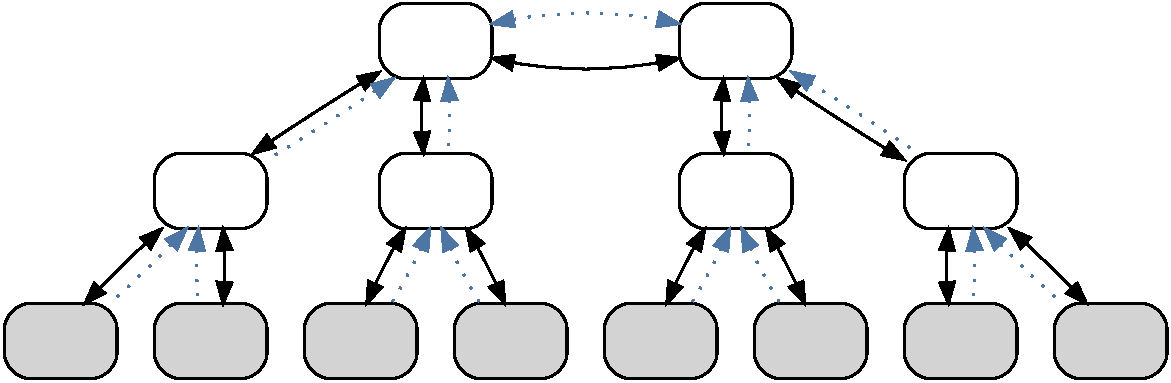
\includegraphics[width=.95\textwidth]{resources/images/example3}
    \caption{Contribution 2 goal}\label{fig:contrib2:goal}
\end{figure}

\sidenote{Approach}
\todomid{write}

\subsection{First Part}

\sidenote{Overview}
\todomid{write}

\sidenote{Approach}
\todomid{write}

\sidenote{Integration}
\todomid{write}

\subsection{Second Part}

\sidenote{Overview}
\todomid{write}

\sidenote{Approach}
\todomid{write}

\sidenote{Integration}
\todomid{write}

\subsection{Third Part}

\sidenote{Overview}
\todomid{write}

\sidenote{Approach}
\todomid{write}

\sidenote{Integration}
\todomid{write}

\section{Conclusion}

\sidenote{Summary}
\todomid{write}

\sidenote{Takeaway 1}
\todomid{write}

\sidenote{Takeaway 2}
\todomid{write}

\sidenote{Takeaway 3}
\todomid{write}

\sidenote{Next chapter}
\todomid{write}

%    \cleardoublepage
\chapter{Contribution 3}\label{sec:contrib3}\minitoc\vspace{.5cm}
\index{Contribution 3}

\section{Introduction}

\begin{wrapfigure}{r}{0.2\textwidth}
    \centering
    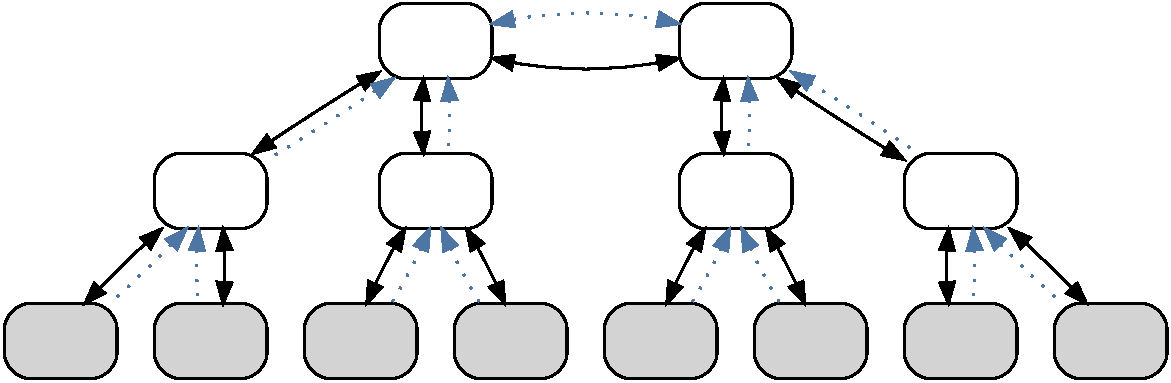
\includegraphics[width=0.2\textwidth]{resources/images/example3}
\end{wrapfigure}

\sidenote{Overview}
\todomid{write}

\sidenote{Structure of Research}
\todomid{write about \Cref{fig:hourglass:contrib3}}

\begin{figure}[H]
    \centering
    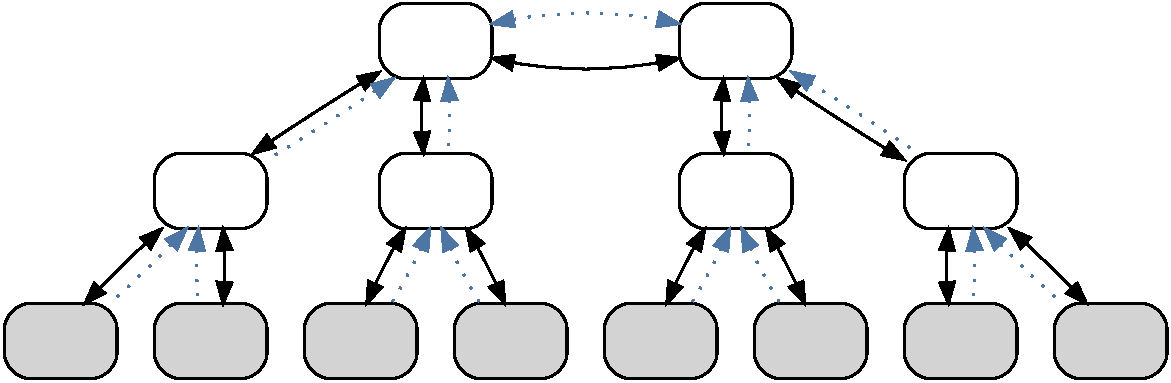
\includegraphics[width=.55\textwidth]{resources/images/example3}
    \caption{Placement of Contribution 3 in the structure of research}\label{fig:hourglass:contrib3}
\end{figure}

\section{State of the Art}

\sidenote{Overview}
\todomid{write about \Cref{fig:contrib3:related}}

\begin{figure}[htbp]
    \centering
    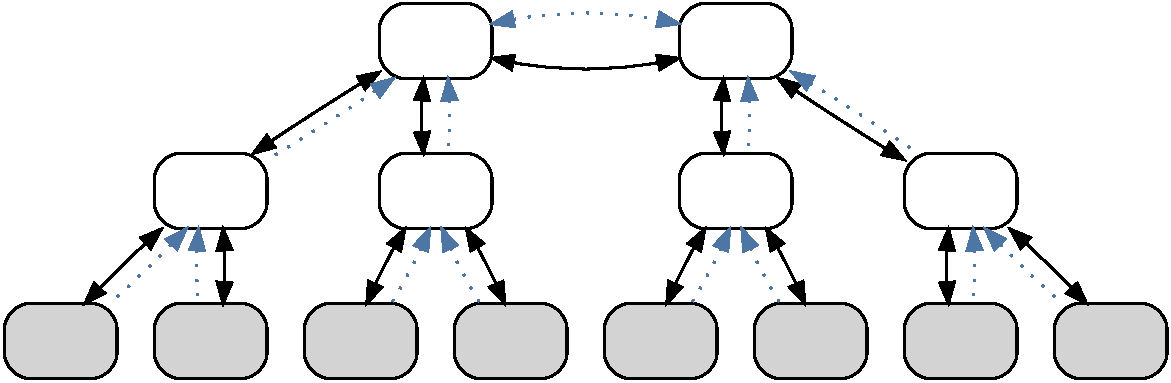
\includegraphics[width=.6\textwidth]{resources/images/example3}
    \caption{Relationship of Contribution 3 to related work}\label{fig:contrib3:related}
\end{figure}

\subsection{Related Work 1}

\sidenote{Overview}
\todomid{write}

\sidenote{Some Aspects}
\todomid{write}

\sidenote{Issues}
\todomid{write about \Cref{lst:contrib3:rw1}}

\lstset{caption=Listing related to related work 1 for Contribution 3, label=lst:contrib3:rw1,
language=xml, breaklines=true, numbers=left, basicstyle=\small\ttfamily,
stepnumber=1, frame=single, inputencoding=utf8/latin1}~\lstinputlisting{resources/code/example.java}

\subsection{Related Work 2}

\sidenote{Overview}
\todomid{write}

\sidenote{Some Aspects}
\todomid{write}

\sidenote{Issues}
\todomid{write about \Cref{lst:contrib3:rw2}}

\lstset{caption=Listing related to related work 2 for Contribution 3, label=lst:contrib3:rw2,
language=xml, breaklines=true, numbers=left, basicstyle=\small\ttfamily,
stepnumber=1, frame=single, inputencoding=utf8/latin1}~\lstinputlisting{resources/code/example.java}

\subsection{Related Work 3}

\sidenote{Overview}
\todomid{write}

\sidenote{Some Aspects}
\todomid{write}

\sidenote{Issues}
\todomid{write about \Cref{lst:contrib3:rw3}}

\lstset{caption=Listing related to related work 3 for Contribution 3, label=lst:contrib3:rw3,
language=xml, breaklines=true, numbers=left, basicstyle=\small\ttfamily,
stepnumber=1, frame=single, inputencoding=utf8/latin1}~\lstinputlisting{resources/code/example.java}


\section{Own Approach}

\subsection{Overview}

\sidenote{Intro}
\todomid{write}

\sidenote{Goal}
\todomid{write about \Cref{fig:contrib3:goal}}

\begin{figure}[htbp]
    \centering
    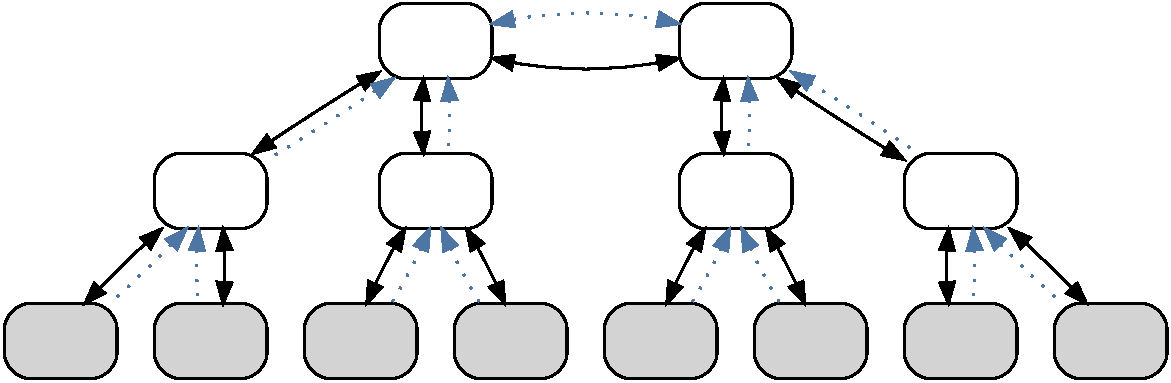
\includegraphics[width=.95\textwidth]{resources/images/example3}
    \caption{Contribution 3 goal}\label{fig:contrib3:goal}
\end{figure}

\sidenote{Approach}
\todomid{write}

\subsection{First Part}

\sidenote{Overview}
\todomid{write}

\sidenote{Approach}
\todomid{write}

\sidenote{Integration}
\todomid{write}

\subsection{Second Part}

\sidenote{Overview}
\todomid{write}

\sidenote{Approach}
\todomid{write}

\sidenote{Integration}
\todomid{write}

\subsection{Third Part}

\sidenote{Overview}
\todomid{write}

\sidenote{Approach}
\todomid{write}

\sidenote{Integration}
\todomid{write}

\section{Conclusion}

\sidenote{Summary}
\todomid{write}

\sidenote{Takeaway 1}
\todomid{write}

\sidenote{Takeaway 2}
\todomid{write}

\sidenote{Takeaway 3}
\todomid{write}

\sidenote{Next chapter}
\todomid{write}

%    \cleardoublepage
\chapter{Evaluation}\label{sec:eval}\minitoc\vspace{.5cm}
\index{Evaluation}\index{Validation}\index{Verification}

\section{Introduction}

\begin{wrapfigure}{r}{0.2\textwidth}
    \centering
    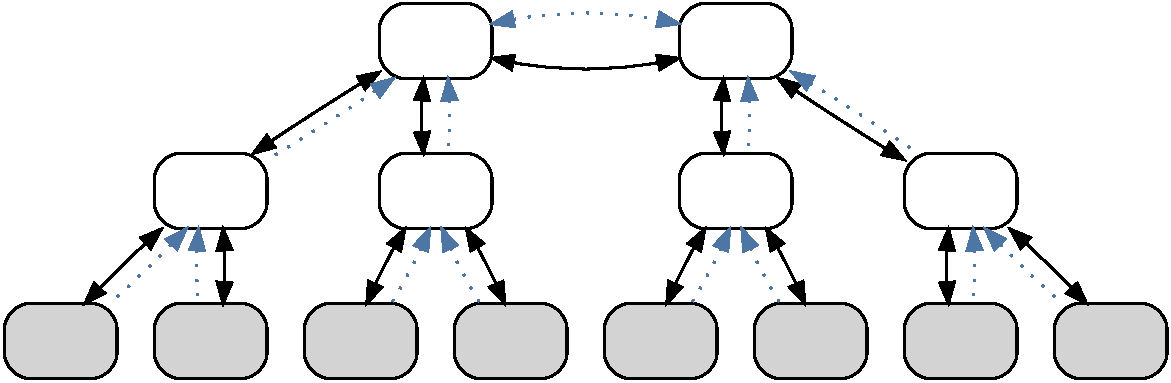
\includegraphics[width=0.2\textwidth]{resources/images/example3}
\end{wrapfigure}

\sidenote{Overview}
\todomid{write about \Cref{sec:eval:tec}}

\begin{figure}[htbp]
    \centering
    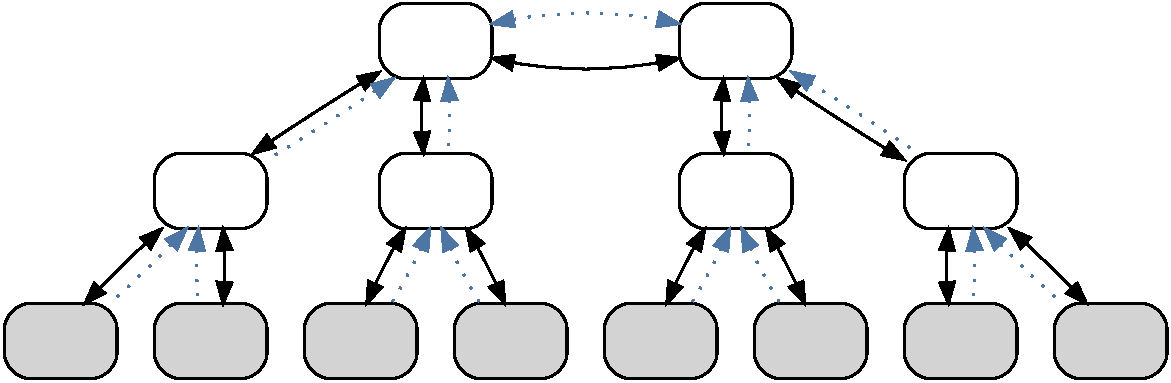
\includegraphics[width=.8\textwidth]{resources/images/example3}
    \caption{Choice of verification and validation techniques~\cite{li2002design}}\label{sec:eval:tec}
\end{figure}

\sidenote{Approaches}
\todomid{write}

\sidenote{Structure of Research}
\todomid{write about \Cref{fig:hourglass:evaluation}}

\begin{figure}[htpb]
    \centering
    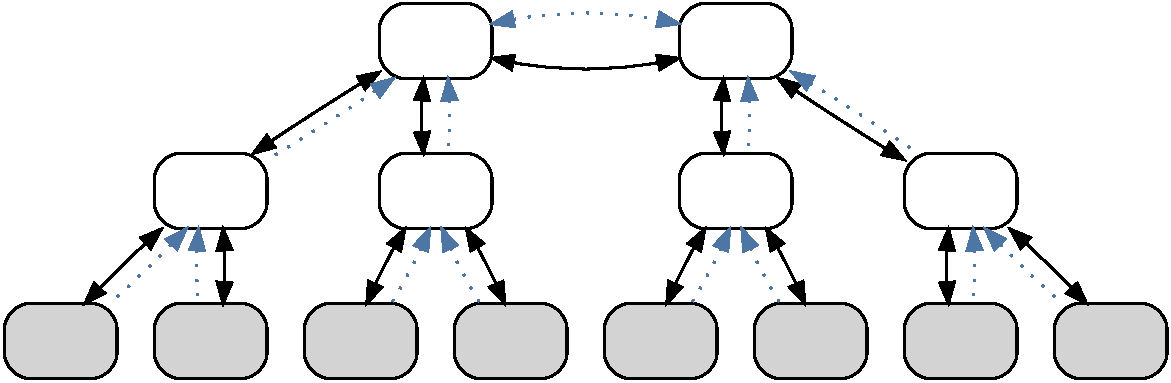
\includegraphics[width=.55\textwidth]{resources/images/example3}
    \caption{Placement of the evaluation in the structure of research}\label{fig:hourglass:evaluation}
\end{figure}

\section{Experimental Validation}

\sidenote{Overview}
\todomid{write about \Cref{tbl:eval:experiments}}

\begin{sidewaystable}
      \centering
      \captionsetup{type=table}
      \caption{Sideways table}
      \begin{tabular}{lllllll}\toprule
  \textbf{Experiment 1}   & \textbf{Experiment 2}  & \textbf{Experiment 3} & \textbf{Experiment 4} & \textbf{Experiment 5} & \textbf{Experiment 6} & \textbf{Experiment 7}  \\ \midrule
  CATCH & ME & IF & YOU & CAN & \emph{NOW} & OR NEVER \\
  CATCH & ME & IF & YOU & CAN & \emph{NOW} & OR NEVER \\
  CATCH & ME & IF & YOU & CAN & \emph{NOW} & OR NEVER \\
  CATCH & ME & IF & YOU & CAN & \emph{NOW} & OR NEVER \\
  CATCH & ME & IF & YOU & CAN & \emph{NOW} & OR NEVER \\
  CATCH & ME & IF & YOU & CAN & \emph{NOW} & OR NEVER \\
  CATCH & ME & IF & YOU & CAN & \emph{NOW} & OR NEVER \\
  CATCH & ME & IF & YOU & CAN & \emph{NOW} & OR NEVER \\
  CATCH & ME & IF & YOU & CAN & \emph{NOW} & OR NEVER \\
  CATCH & ME & IF & YOU & CAN & \emph{NOW} & OR NEVER \\
  CATCH & ME & IF & YOU & CAN & \emph{NOW} & OR NEVER \\
  \bottomrule
      \end{tabular}\label{tbl:eval:experiments}
\end{sidewaystable}


\subsection{Setup 1}

\sidenote{Overview}
\todomid{write}

\sidenote{Integration}
\todomid{write about \Cref{eq:var_idb}}

\small
\begin{equation}
  \begin{array}{l}
    \displaystyle t^{p_d}_{fw}(d) = \max_{d}(t_{child_{i}}) \\
    \displaystyle t^{p_d}_{db}(d) = \sum_{i=1}^{d} t_{db_{i}} \\
    \displaystyle t^{p_d}_{pc}(n,d) =
    	\begin{cases}
        	t_{pc}(d) + c(n) & \text{if $d = 1$,}\\
        	t_{pc}(d) + c(n) + \max(t_{avail}(d)) & \text{if $d>1$.}\\
        \end{cases}
  \end{array}\label{eq:var_idb}
\end{equation}
\normalsize

\sidenote{Example}
\todomid{write about \Cref{lst:eval:exp1}}

\needspace{5\baselineskip}\lstset{caption=Experiment 1, label=lst:eval:exp1,
language=ttl, breaklines=true, numbers=left,
stepnumber=1, frame=single, inputencoding=utf8/latin1}~\lstinputlisting{resources/code/example.java}

\subsection{Setup 2}

\sidenote{Overview}
\todomid{write}

\sidenote{Integration}
\todomid{write}

\sidenote{Example}
\todomid{write about \Cref{fig:eval:sub1,fig:eval:sub2,fig:eval:sub}}

\begin{figure}
    \begin{subfigure}[b]{.455\textwidth}
      \centering
      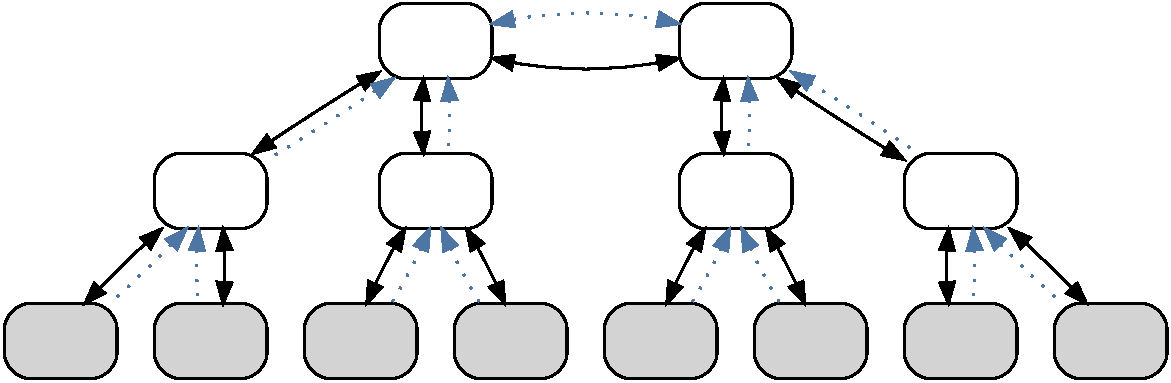
\includegraphics[width=.9\textwidth,frame]{resources/images/example3}
      \caption{Subfig 1}\label{fig:eval:sub1}
    \end{subfigure}~\begin{subfigure}[b]{.545\textwidth}
      \centering
      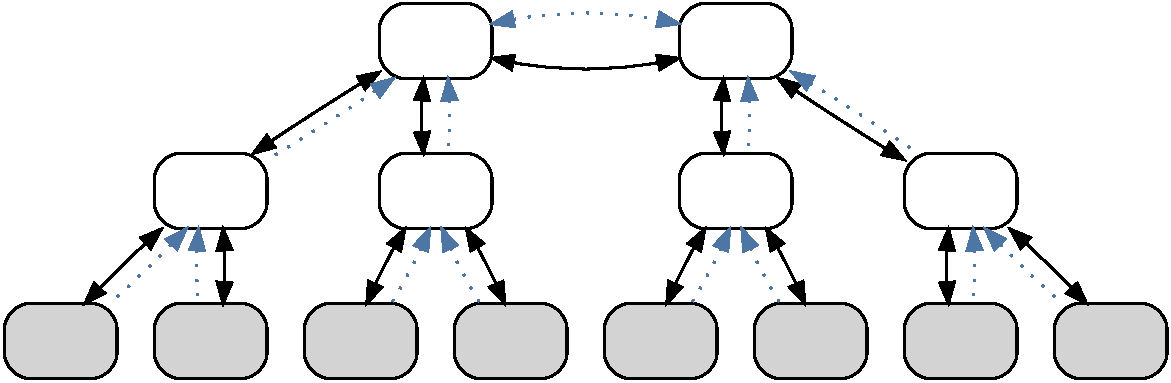
\includegraphics[width=1\textwidth,frame]{resources/images/example3}
      \caption{Subfig 2}\label{fig:eval:sub2}
    \end{subfigure}
    \caption{Sub Figures}\label{fig:eval:sub}
\end{figure}


\section{Performance Evaluation}

\sidenote{Overview}
\todomid{write}

\subsection{Evaluation 1}

\sidenote{Setup}
\todomid{write}

\sidenote{Cost Metrics}
\todomid{write}

\sidenote{Optimizing}
\todomid{write}

\sidenote{Performance Comparison}
\todomid{write}

\subsection{Evaluation 2}

\sidenote{Setup}
\todomid{write}

\sidenote{Response Times}
\todomid{write}
\begin{itemize}[noitemsep]
  \item \emph{In}: 159 ms $\pm$ 21 ms (95\% CI)
  \item \emph{Out}: 33 ms $\pm$ 5 ms (95\% CI)
  \item \emph{Between}: 238 ms $\pm$ 9 ms (95\% CI)
  \item \emph{After}: 45 ms $\pm$ 1 ms (95\% CI)
  \item \emph{Under}: 215 ms $\pm$ 2 ms (95\% CI)
  \item \emph{Over}: 148 ms $\pm$ 3 ms (95\% CI)
\end{itemize}

\sidenote{Scalability}
\todomid{write}

\section{Observational Validation}

\sidenote{Overview}
\todomid{write}

\subsection{Project 1}

\sidenote{Overview}
\todomid{write}

\sidenote{System Specification}
\todomid{write}

\sidenote{Extraction}
\todomid{write}

\sidenote{Example}
\todomid{write}

\subsection{Project 2}

\sidenote{Overview}
\todomid{write}

\sidenote{System Specification}
\todomid{write about \Cref{fig:eval:side}}

\begin{figure}[htbp]
    \centering
    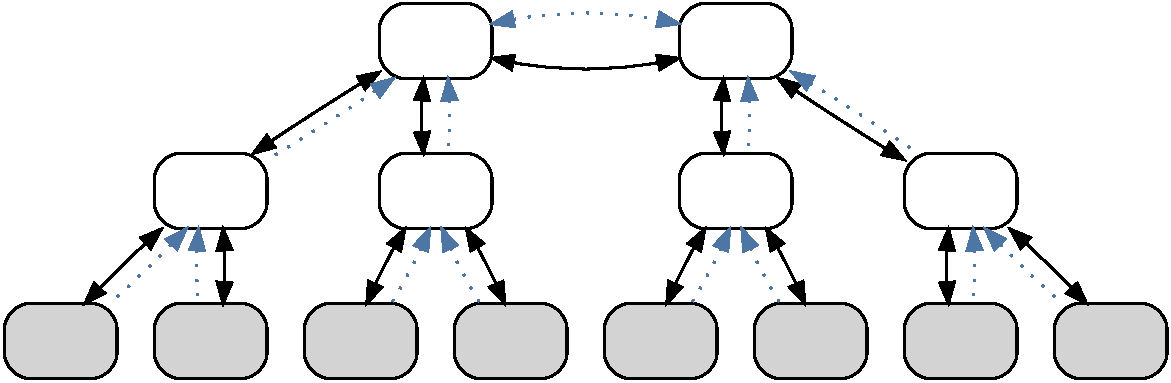
\includegraphics[height=.5\textwidth,angle=270]{resources/images/example3}
    \caption{Sideways figure}\label{fig:eval:side}
\end{figure}

\sidenote{Extraction}
\todomid{write}

\sidenote{Example}
\todomid{write}

\section{Deployments}

\sidenote{Overview}
\todomid{write}

\subsection{Installation 1}

\sidenote{Overview}
\todomid{write}

\sidenote{Integration}
\todomid{write}


\subsection{Installation 2}

\sidenote{Overview}
\todomid{write}

\sidenote{Integration}
\todomid{write}

\section{Code Verification}

\sidenote{Overview}
\todomid{write}

\sidenote{Static Tests}
\todomid{write}

\sidenote{Continuous Integration}
\todomid{write}

\sidenote{Test Coverage}
\todomid{write}

\section{Comparative Analysis}

\sidenote{Overview}
\todomid{write}

\subsection{Requirement Evaluation}

\sidenote{\Cref{tbl:reqs:compare}}
\todomid{write}

\begin{tabularx}{\textwidth}{p{2cm}X}
    \caption{Mapping requirements against own approach}\label{tbl:reqs:compare}\\
    \toprule
    \textbf{Requirements}& \textbf{Approach}  \\\midrule
    \endfirsthead%
    \toprule
    \textbf{Requirements}& \textbf{Approach}  \\\midrule
    \endhead%
\ref{req:stakeholder1:foo}\newline(Foo) &
\todomid{write}
\\\midrule

\ref{req:stakeholder1:bar}\newline(Bar) &
\todomid{write}
\\\midrule

\ref{req:stakeholder2:foo}\newline(Foo) &
\todomid{write}
\\\midrule

\ref{req:stakeholder2:bar}\newline(Bar) &
\todomid{write}
\\\midrule

\ref{req:stakeholder3:foo}\newline(Foo) &
\todomid{write}
\\\midrule

\ref{req:stakeholder3:bar}\newline(Bar) &
\todomid{write}

\\\bottomrule
\end{tabularx}

\subsection{Comparison with Other Approaches}

\sidenote{Overview}
\todomid{write}

\sidenote{\Cref{tbl:approaches:compare}}
\todomid{write about \Cref{tbl:approaches:compare}}

\begin{tabularx}{\textwidth}{p{2cm}LLLLLL}
    \caption{Comparison of related work with own approach}\label{tbl:approaches:compare}\\
    \toprule
    \textbf{Requirements} & \textbf{Related 1} & \textbf{Related 2} & \textbf{Related 3} & \textbf{Related 4} & \textbf{Related 5} & \textbf{Own Approach} \\\midrule
    \endfirsthead%
    \toprule
    \textbf{Requirements} & \textbf{Related 1} & \textbf{Related 2} & \textbf{Related 3} & \textbf{Related 4} & \textbf{Related 5} & \textbf{Own Approach} \\\midrule
    \endhead%

\ref{req:stakeholder1:foo}~\ref{req:stakeholder1:bar} & \textbf{(+)} & \textbf{(++)} & \textbf{(o)} & \textbf{(-)} & \textbf{(o)} & \textbf{(+++)} \\
(\ac{ABAC}) & \ac{ABAC} \ac{ABAC} v3, \ac{ABAC} \ac{ABAC} & \ac{ABAC} \ac{ABAC} v2, \ac{ABAC}, native \ac{ABAC} & \ac{ABAC} & native \ac{ABAC} & \ac{ABAC} \ac{ABAC} v2 & \ac{ABAC} \ac{ABAC} v3, \ac{ABAC} \ac{ABAC}, \ac{ABAC}, native \ac{ABAC}, native \\\midrule

\ref{req:stakeholder3:foo} & \textbf{(o)} & \textbf{(++)} &  & & \textbf{(++)} & \textbf{(+)} \\
(Details) & via foo & by bar / role-foo & --- & --- & bar / foo & foo-bar \\\midrule

\ref{req:stakeholder2:foo}~\ref{req:stakeholder2:bar}~\ref{req:stakeholder3:bar} & \textbf{(+)} & \textbf{(+)} & & \textbf{(+)} & \textbf{(+)} & \textbf{(+)} \\
(Barli) & via barli & via fooli & --- & via bar-foo & via foo-bar & via bar-bar \\\bottomrule
\end{tabularx}

\section{Conclusion}

\sidenote{Summary}
\todomid{write}

\sidenote{Takeaway 1}
\todomid{write}

\sidenote{Takeaway 2}
\todomid{write}

\sidenote{Takeaway 3}
\todomid{write}

\sidenote{Next chapter}
\todomid{write}

%    \cleardoublepage
\chapter{Summary and Further Work}\minitoc\label{sec:summary}\vspace{.5cm}

\section{Overview}

\begin{wrapfigure}{r}{0.2\textwidth}
    \centering
    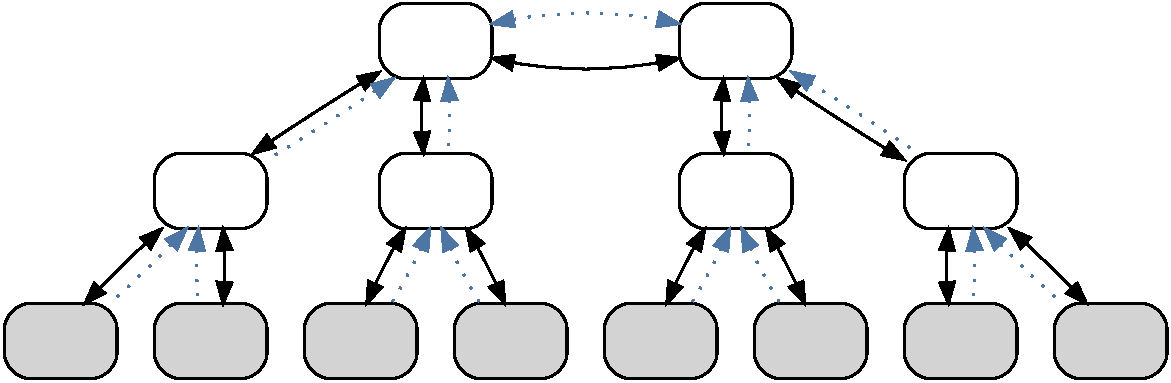
\includegraphics[width=0.2\textwidth]{resources/images/example3}
\end{wrapfigure}

\sidenote{Contributions}
\todomid{write}

\begin{figure}
    \centering
    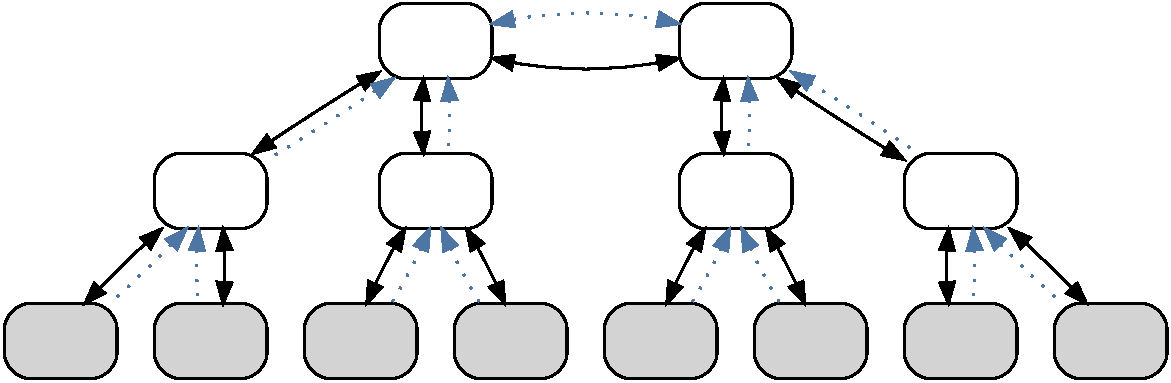
\includegraphics[width=.55\textwidth]{resources/images/example3}
    \caption{Placement of the outlook in the structure of research}\label{fig:hourglass:outlook}
\end{figure}

\sidenote{Dissemination}
\todomid{write about \Cref{fig:hourglass:outlook}}

\section{Conclusions and Impact}

\sidenote{Context}
\todomid{write}

\sidenote{Contribution 1}
\todomid{write}

\sidenote{Contribution 2}
\todomid{write}

\sidenote{Contribution 3}
\todomid{write}

\section{Outlook}

\sidenote{Intro}
\todomid{write}

\sidenote{Application Area 1}
\todomid{write about \Cref{fig:outlook:aa1}}

\begin{figure}
    \centering
    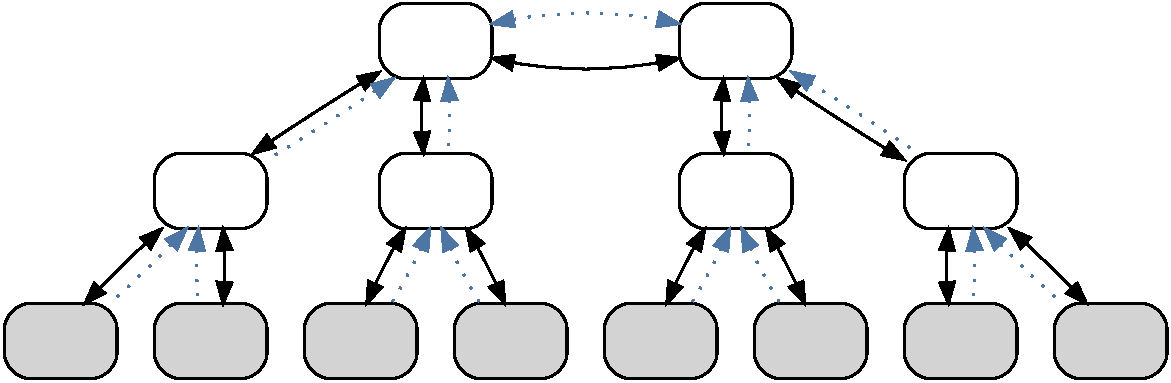
\includegraphics[width=.85\textwidth]{resources/images/example3}
    \caption{Area 1~\cite{li2002design}}\label{fig:outlook:aa1}
\end{figure}

\sidenote{Application Area 2}
\todomid{write}

\sidenote{Application Area 3}
\todomid{write}

\sidenote{Application Area 4}
\todomid{write}

    \nolinenumbers
    \cleardoublepage
%------------------------------
% APPENDIX
%------------------------------
    \appendix
    \pagenumbering{Roman}
    \setcounter{page}{1}
    \cleardoublepage\chapter{Specifications}\minitoc\vspace{.5cm}

\section{Specification 1}\index{Specification 1}

\todomid{write about \Cref{lst:spec1}}

\lstset{language=ttl, breaklines=true, caption=Specification 1, %
emptylines=0,
label=lst:spec1, numbers=left, stepnumber=1, inputencoding=utf8}
\lstinputlisting{resources/code/example.java}


\section{Specification 2}\index{Specification 2}

\todomid{write about \Cref{lst:spec2}}

\lstset{language=ttl, breaklines=true, caption=Specification 2, %
emptylines=0,
label=lst:spec2, numbers=left, stepnumber=1, inputencoding=utf8}
\lstinputlisting{resources/code/example.java}


\cleardoublepage\chapter{Test Results}\minitoc\vspace{.5cm}

\section{Conformance Results}

\sidenote{Overview}
\todomid{write about \Cref{fig:test:result1,fig:test:result2}}

\begin{figure}[H]
    \centering
    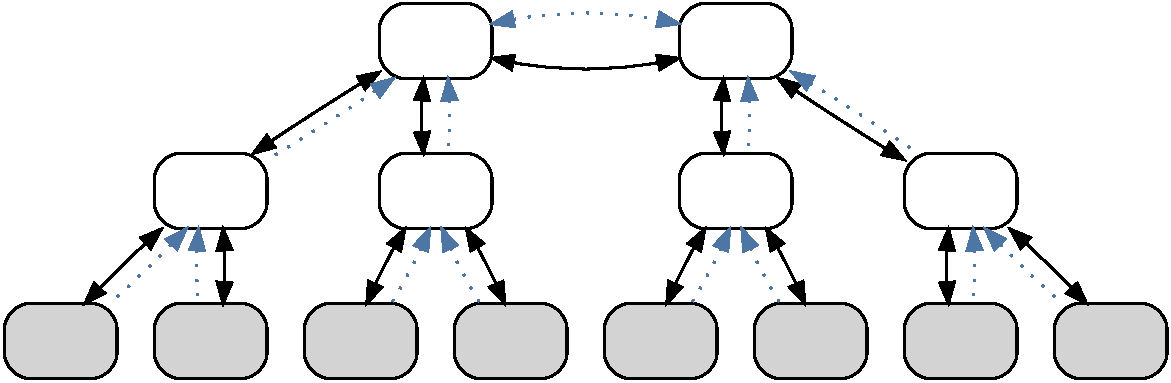
\includegraphics[width=.9\textwidth,frame,page=1]{resources/images/example3}
    \caption{Test results (page 1)}\label{fig:test:result1}
\end{figure}

\begin{figure}[H]
    \centering
    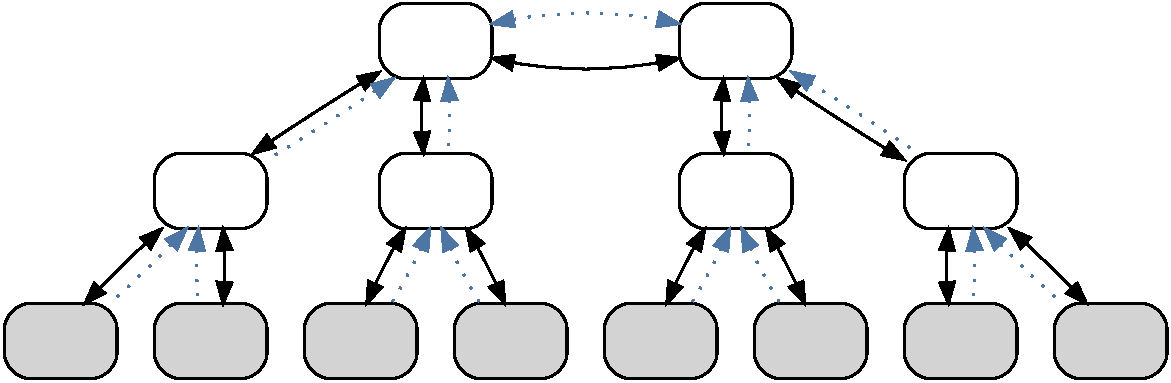
\includegraphics[width=.9\textwidth,frame,page=1]{resources/images/example3}
    \caption{Test results (page 2)}\label{fig:test:result2}
\end{figure}

\section{Performance Results}

\subsection{Histograms}

\sidenote{Overview}
\todomid{write about \Cref{fig:eval:perf:hist:forms}}

\begin{figure}[H]
    \begin{subfigure}[b]{.5\textwidth}
      \centering
      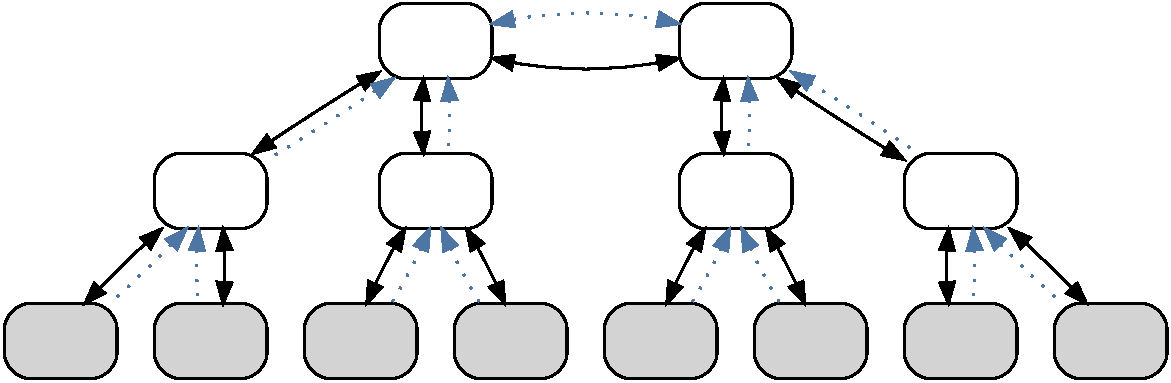
\includegraphics[width=.95\textwidth,frame]{resources/images/example3}
      \caption{Form A}
    \end{subfigure}~\begin{subfigure}[b]{.5\textwidth}
      \centering
      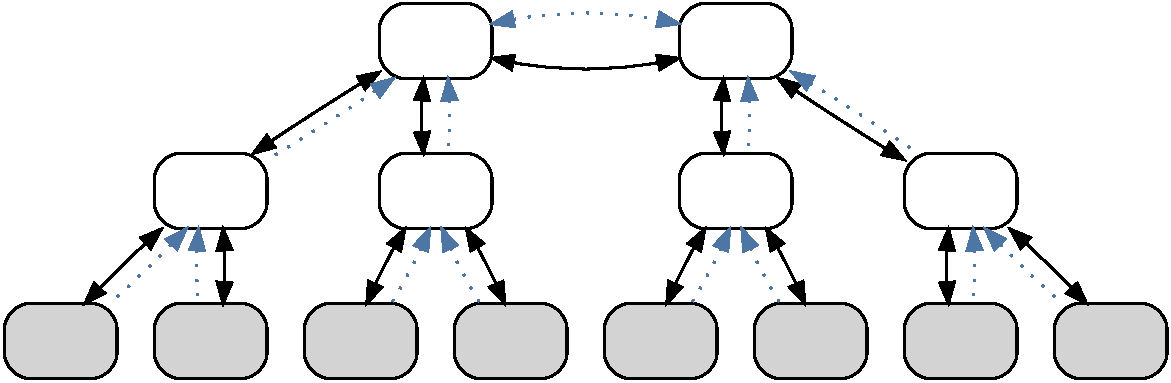
\includegraphics[width=.95\textwidth,frame]{resources/images/example3}
      \caption{Form B}
    \end{subfigure}
    \caption{Histogram of Forms}\label{fig:eval:perf:hist:forms}
\end{figure}


\subsection{Lineplots}

\sidenote{Overview}
\todomid{write about \Cref{fig:eval:perf:line:lines}}

\begin{figure}[H]
    \begin{subfigure}[b]{.5\textwidth}
      \centering
      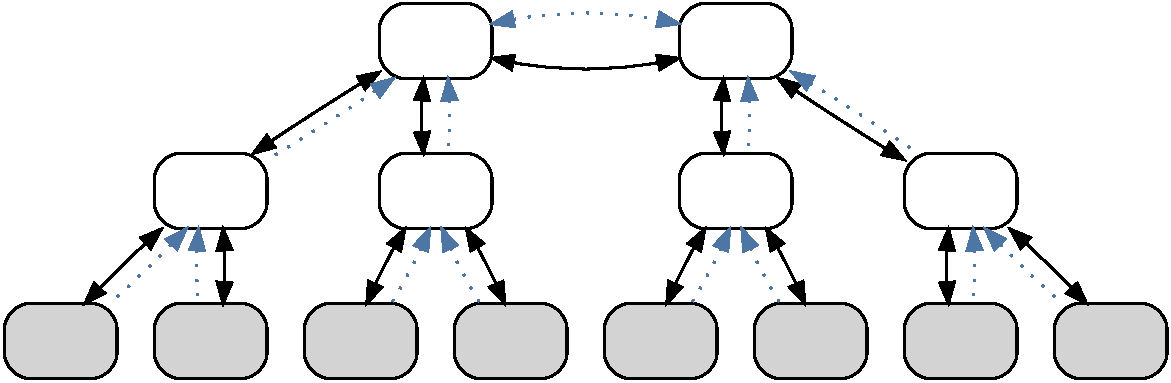
\includegraphics[width=.95\textwidth,frame]{resources/images/example3}
      \caption{Lines A}
    \end{subfigure}~\begin{subfigure}[b]{.5\textwidth}
      \centering
      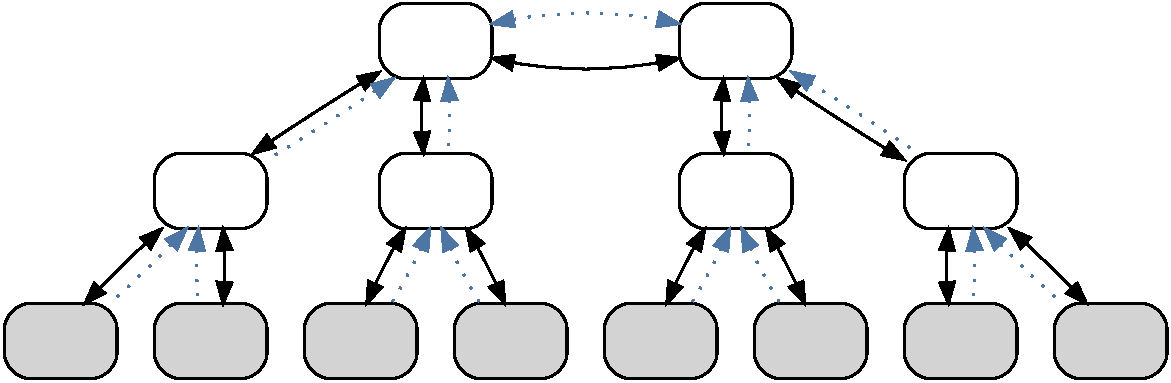
\includegraphics[width=.95\textwidth,frame]{resources/images/example3}
      \caption{Lines A}
    \end{subfigure}
    \caption{Lineplot of the lines}\label{fig:eval:perf:line:lines}
\end{figure}

%------------------------------
% REFERENCES
%------------------------------
    \cleardoublepage
    \cleardoublepage
\chapter*{Acronyms}
\mtcaddchapter\addstarredchapter{Acronyms}
\markboth{Acronyms}{Acronyms}
\stepcounter{chapter}
%\renewcommand*{\chapterthumbformat}{Acronyms}
\begingroup
\let
\newpage
\relax
\printacronyms[exclude=exclude, template = longtable, preamble = {A list of all abbreviations used in this document with a reference to the pages , where used.}]
\endgroup


%\cleardoublepage
%\stepcounter{chapter}
%\renewcommand{\glossaryname}{Glossary}
%\markboth{\glossaryname}{\glossaryname}
%\renewcommand*{\chapterthumbformat}{\glossaryname}
%\printglossary%

\cleardoublepage
\chapter*{Bibliography}
\mtcaddchapter\addstarredchapter{Bibliography}
\markboth{Bibliography}{Bibliography}
\stepcounter{chapter}
%\renewcommand*{\chapterthumbformat}{Bibliography}
%\minitoc\vspace{.5cm}

\section*{List of Author's Publications Covered in this Thesis}
\nocite{li2002design}
\newrefcontext[labelprefix=a]
\printbibliography[keyword=own,heading=empty,category=cited]


\section*{References to Scientific Publications}
\defbibfilter{papers}{
  type=article
  or type=inproceedings
  or type=proceedings
  or type=journal
  or type=phdthesis
  or type=incollection
  or type=book
  or keyword=thesis
  and not keyword=W3C
  and not keyword=RFC
  and not keyword=ITU
  and not keyword=IEEE
  and not keyword=ANSI
  and not keyword=OGF
  and not keyword=web
  and not keyword=presentation
  and not keyword=workingpaper
}
\newrefcontext[labelprefix=p]
\printbibliography[filter=papers,heading=empty,category=cited,notkeyword=own]


\section*{Technical References}

\defbibfilter{standards}{
  type=techreport
  or type=report
  or keyword=W3C
  or keyword=RFC
  or keyword=TMF
  or keyword=ITU
  or keyword=IEEE
  or keyword=ANSI
  or keyword=OGF
  or keyword=ETSI
  or keyword=OneM2M
  or keyword=IETF
  or keyword=OMA
  or keyword=TMG
  or keyword=NIST
  or keyword=SNIA
  or keyword=OMG
  or keyword=DMTF
  or keyword=OASIS
  or keyword=deliverable
  or keyword=techreport
  or keyword=whitepaper
  and not keyword=web
  and not keyword=presentation
  and not keyword=workingpaper
}
\newrefcontext[labelprefix=t]
\printbibliography[filter=standards,heading=empty,category=cited,notkeyword=own]


\section*{Miscellaneous References}
\defbibfilter{misc}{
  keyword=web
  or keyword=presentation
  or keyword=workingpaper
}
\newrefcontext[labelprefix=m]
\printbibliography[filter=misc,heading=empty,category=cited,notkeyword=own]


\section*{Not referenced (will be empty)}
\todo{this section should be empty at the end}
\nocite{*}
\newrefcontext[labelprefix=x]
\printbibliography[heading=empty,notcategory=cited,notkeyword=own]

%------------------------------
% INDEX
%------------------------------
    \backmatter
    \cleardoublepage\cleardoublepage
\phantomsection
\stepcounter{chapter}
\renewcommand{\indexname}{Index}
%\renewcommand*{\chapterthumbformat}{\indexname}
\markboth{\indexname}{\indexname}
\printindex%

%------------------------------
% END DOCUMENT
%------------------------------
\end{document}
% ------------------------------------------------------------------------------
